%%%%%%%%%%%%%%%%%%%%%%%%%%%%%%%%%%%%%%%%%%%%%%%%%%%%%%%%%%%%%%%%%%%%%%%%%%%%%%%%
% TUM-Vorlbrge: Wissenschaftliche Arbeit inkl. Deckblatt
%%%%%%%%%%%%%%%%%%%%%%%%%%%%%%%%%%%%%%%%%%%%%%%%%%%%%%%%%%%%%%%%%%%%%%%%%%%%%%%%
%
% Rechteinhaber:
%     Technische Universität München
%     https://www.tum.de
% 
% Gestaltung:
%     ediundsepp Gestaltungsgesellschaft, München
%     http://www.ediundsepp.de
% 
% Technische Umsetzung:
%     eWorks GmbH, Frankfurt am Main
%     http://www.eworks.de
%
% Angepasst für Heinz Nixdorf-Lehrstuhl für Biomedizinische Elektronik (Version 2017/11/29)
%
%%%%%%%%%%%%%%%%%%%%%%%%%%%%%%%%%%%%%%%%%%%%%%%%%%%%%%%%%%%%%%%%%%%%%%%%%%%%%%%%

%%%%%%%%%%%%%%%%%%%%%%%%%%%%%%%%%%%%%%%%%%%%%%%%%%%%%%%%%%%%%%%%%%%%%%%%%%%%%%%%
\documentclass[%
    fontsize=11pt, % Schriftgröße
    twoside=on % kein einseitiges Layout
]{scrbook} % Dokumentenklasse: KOMA-Script Book
\usepackage{scrlayer-scrpage} % Anpassbare Kopf- und Fußzeilen

\usepackage[utf8]{inputenc} % Textkodierung: UTF-8
\usepackage[T1]{fontenc} % Zeichensatzkodierung
\usepackage{csquotes}

\usepackage[ngerman, english]{babel} % Deutsche Lokalisierung
\usepackage{graphicx} % Grafiken
\usepackage{wrapfig} % Text an Bilder und Tabellen vorbeifließen lassen
\usepackage{siunitx} % SI Units 
\usepackage{lscape} % Portrait- oder Landscape ausrichtung
\usepackage[absolute]{textpos} % Positionierung
\usepackage{amsmath}
\usepackage{amssymb}

% Schriftart Helvetica:
\usepackage[scaled]{helvet}
\renewcommand{\familydefault}{\sfdefault}

% TUM Schriftfarbe:
\usepackage{color} %Schriftfarbe
\definecolor{TUMblau}{RGB}{0, 82, 147}

\usepackage{calc} % Berechnungen
\usepackage{tabto} % Tabulatoren
\usepackage{parskip}

% Silbentrennung:
\usepackage{hyphenat}
\hyphenation{TUM in-te-res-siert} % Eigene Silbentrennung
%\tolerance 2414
%\hbadness 2414
%\emergencystretch 1.5em
%\hfuzz 0.3pt
%\widowpenalty=10000     % Hurenkinder
%\clubpenalty=10000      % Schusterjungen
%\vfuzz \hfuzz

\usepackage[hidelinks]{hyperref} % Hyperlinks
\usepackage[onehalfspacing]{setspace} % 1,5facher Zeilenabstand
\usepackage{calc} % Berechnungen
\usepackage{enumitem} % Mehr Kontrolle über itemize-, enumerate- und description-Umgebungen
\usepackage{relsize} % Schriftgröße in Abhängigkeit von aktueller anpassen
\usepackage{tabularx} % Flexiblere Tabellen
\usepackage{caption} % Anpassen von Beschriftungen

% Nummerierung von Abbildungen & Tabellen durchgängig, statt nach Kapiteln:
%\usepackage{tocloft}
\usepackage{chngcntr}
\counterwithout{figure}{chapter}
\counterwithout{table}{chapter}

% Abkürzungen, Glossare:
\usepackage[%
%    xindy,% xindy zum Indexieren verwenden
    acronym,% Separates Akronym-Verzeichnis
    nopostdot,% Kein Punkt am Ende einer Beschreibung im Glossar
    nomain,
    automake, 
    nonumberlist,
]{glossaries}

% Debugging:
%\usepackage{showframe} % Layout-Boxen anzeigen
%\usepackage{layout} % Layout-Informationen
%\usepackage{printlen} % Längenwerte ausgeben



%% Neue Pakete
\usepackage{subcaption}

\usepackage{stackengine}
\usepackage{tikz}
\usepackage{svg}
\usepackage{pgfkeys}

\usepackage[ backend=biber,
%style=ieee,
style=numeric-comp,
natbib=true,
sorting=none,
%sortcites = true,
url=false, 
doi=true,
eprint=false]{biblatex}

\usepackage{lipsum}
\sisetup{detect-all,
%	per-mode=fraction,
%	parse-numbers=false
	separate-uncertainty=true,
	multi-part-units=single
}
\DeclareSIUnit\particle{particle}
\DeclareSIUnit\Ferrum{Fe}
\DeclareSIUnit\sccm{sccm}
\DeclareSIUnit\torr{Torr}
\DeclareSIUnit\molar{M}
\DeclareSIUnit\rpm{rpm}
\DeclareSIUnit{\dyne}{dyne}


\DeclareSIUnit[number-unit-product = {}]{\inch}{\textquotedbl}
\newcolumntype{R}{>{\raggedright\arraybackslash}X}
\newcolumntype{C}{>{\centering\arraybackslash}X} % Automatische Texttrennung in Tabellen
\usepackage{cancel}
\usepackage{listings}
\lstset{
language=Matlab,
showstringspaces = false}


%% MATH and CHEM typesetting
\usepackage{chemmacros} % Chemical formulae
\usepackage[capitalize]{cleveref}
\usepackage{esvect} %% Fine vector arrows
\usepackage{abraces} % Braces under and over text
\usepackage{scalerel} % Get smaller subscripts

\usepackage{booktabs} % get fancy table lines

%% Debug only figures
%\usepackage[active,tightpage]{preview}
%\PreviewSnarfEnvironment[{[]}]{figure} % !!! NICHT ENTFERNEN !!!
%%%%%%%%%%%% GMR STUFF
\glsnoexpandfields 

\newacronym{gmr}{GMR}{giant magneto resistance}

\newacronym{mr}{MR effect}{magneto-resistive effect}

\newacronym{pdms}{PDMS}{\iupac{poly(dimethylsiloxane)}}

\newacronym{sin}{Si$_\text{3}$N$_\text{4}$}{\iupac{silicon nitride}}

\newacronym{alox}{Al$_\text{2}$Ox$_\text{3}$}{\iupac{aluminium oxide}}

\newacronym{fm}{FM}{Ferrimagnetism}

\newacronym{pm}{PM}{Paramagnetism}

\newacronym{afm}{AFM}{Anti-Ferromagnetism}

\newacronym{nfm}{NFM}{non-ferro-magnetic}

\newacronym{spm}{SPM}{superparamagnetism}

\newacronym{aaf}{AAF}{artificial Anti-Ferromagnet}

\newacronym[longplural={magnetic nanoparticles}]{mnp}{MNP}{magnetic nanoparticle}

\newacronym{el:vp}{V$_\text{p}$}{peak voltage}

\newacronym{el:vpp}{V$_\text{pp}$}{peak-to-peak voltage}

\newacronym{pcb}{PCB}{printed circuit board}

\newacronym{fwhm}{FWHM}{full width at half maximum}

\newacronym{m}{$\protect\mathbf{m}$}{magnetic dipole moment}

\newacronym{M}{$\protect\mathbf{M}$}{magnetization}

\newacronym{B}{$\protect\mathbf{B}$}{magnetic flux density}

\newacronym[longplural={magnetic susceptibilites}, shortplural={$\chi$}]{chi}{$\chi$}{magnetic susceptibility}

\newacronym{snr}{SNR}{signal-to-noise ratio}

\newacronym{rsquadj}{adj. $R^2$}{adjusted coefficient of determination}

\newacronym{chanL}{$l$}{channel length}

\newacronym{chanW}{$w$}{channel width}

\newacronym{chanH}{$h$}{channel height}



%%%%%%%%%%%% Biology %%%%%%%%%%%%%%%%%%%%%%%%%%%%%%%%%


\newacronym{rbc}{RBC}{red blood cell}

\newacronym{pe}{PE}{phycoerythrin}

\newacronym{sem}{SEM}{standard error of the mean}

\newacronym{edta}{EDTA}{\iupac{2,\-2',\-2'',\-2'''-\-(ethane-\-1,2-\-diyl\-dinitrilo)\-tetra\-acetic acid}}


%%%%%%%%%%%%% CEHMISTRY%%%%%%%%%%%%%%%%%

\newacronym{piranha}{piranha}{a mixture from hydrogen peroxide with excess of sulfuric acid}

\newacronym{ipa}{IPA}{isopropanol}

\newacronym{pbs}{PBS}{phosphate buffered saline}

\newacronym{macs}{MACS}{MACS running buffer}

\newacronym{hcl}{HCl}{hydrochloric acid}

\newacronym{h2so4}{H$_\text{2}$SO$_\text{4}$}{sulfuric acid}

\newacronym{sma}{SMA}{styrene maleic anhydride}

\newacronym{uf}{$\text{\mu}$F}{microfluidic}

\newacronym{dih2o}{diH$_\text{2}$O}{deionized water}

\newacronym{n2}{N$_\text{2}$}{nitrogen gas}

\newacronym{o2}{O$_\text{2}$}{oxygen gas}

\newacronym{etoh}{EtOH}{ethanol}

\newacronym{meoh}{MeOH}{methanol}

\newacronym{acoh}{AcOH}{acetic acid}

\newacronym{hf}{HF}{hydrofluoric acid}

\newacronym{h2o2}{H$_\text{2}$O$_\text{2}$}{hydrogen peroxide}

\newacronym{h2so5}{H$_\text{2}$SO$_\text{5}$}{Caro's acid}

\newacronym{aptes}{APTES}{\iupac{3-triethoxy\-silyl\-propan-\-1-\-amine}}

\newacronym{paa}{PAA}{\iupac{poly(acrylic) acid}}

\newacronym{edc}{EDC}{\iupac{3-(Ethyl\-imino\-methylene\-amino)-\-N,N-\-dimethyl\-propan-\-1-\-amine}}

\newacronym{nhs}{NHS}{\iupac{1-Hydroxy-2,5-pyrrolidinedione}}

\newacronym{snhs}{sulfo-NHS}{\iupac{1-hydroxy-2,5-dioxopyrrolidine-3-sulfonate}}

\newacronym{peg}{PEG}{\iupac{poly\-(oxy\-ethylene)}}

\newacronym{mes}{MES}{\iupac{2-(N-morpho\-lino)\-ethane\-sulfonic acid}}

\newacronym{mest}{MEST}{MES buffer with Tween 20}

\newacronym{sam}{SAM}{self-assembled monolayer}

\newacronym{siloxane}{siloxane}{\protect\ch{Si\protect\bond{sb}O\protect\bond{sb}Si}}

\newacronym{silanol}{silanol}{Si\protect\ch{\protect\bond{sb}OH}}

\newacronym{hydroxyl}{hydroxyl}{\protect\ch{\protect\bond{sb}OH}}

\newacronym{amine}{amine}{\protect\ch{\protect\bond{sb}NH2}}

\newacronym{carboxyl}{carboxyl}{\protect\ch{\protect\bond{sb}COOH}}

\newacronym{amide}{carboxamide}{\protect\ch{R1\protect\bond{sb}CONH\protect\bond{sb}R2}}

\newacronym{methylene}{methylene}{\protect\ch{\protect\bond{sb}CH2\protect\bond{sb}}}

\newacronym{ethoxy}{ethoxy}{\protect\ch{\protect\bond{sb}O\protect\bond{sb}CH2\protect\bond{sb}CH3}}

\newacronym{dmso}{DMSO}{\iupac{dimethyl sulfoxide}}

\newacronym{pbst}{PBST}{PBS with Tween 20}

\newacronym{kd}{K$_\text{d}$}{dissociation constant}


%%%%%%%%% MODELLING
\newacronym{t}{$\protect\mathbf{T}_\text{crit}$}{critical tension}

\newacronym{nse}{NSE}{Navier-Stokes-Equation}

\newacronym{u}{$\protect\mathbf{u}$}{flow field}

\newacronym{umean}{$\protect\overline{\protect\mathbf{u}}$}{mean fluid velocity}

\newacronym{q}{$Q$}{flow rate}

\newacronym{a}{$A$}{area}

\newacronym{vc}{$v_\text{c}$}{bead velocity}

\newacronym{dgmr}{$d_\text{GMR}$}{GMR bridge distance}

\newacronym{fs}{$f_\text{s}$}{sampling frequency}

\newacronym{corrVel}{$C_\text{velocity}$}{velocity correction factor}

\newacronym{corrConst}{$C_\text{const}$}{linear fit correction factor}

\newacronym{corrRoll}{$C_\text{rr}$}{rolling resistance factor}

\newacronym{omega_rot}{$\protect\mathbf{\Omega}$}{rotation vector}

\newacronym{omega_freq}{$\omega$}{angular rotation frequency}

\newacronym{surfnormal}{$\protect\vv{n}$}{unit outward normal}

\newacronym{rho}{$\rho$}{density}

\newacronym{eta}{$\eta$}{dynamic viscosity}

\newacronym{u:s}{$\protect\mathbf{u}_\text{s}$}{sedimentation velocity}

\newacronym{bodyforce}{$\sum_\text{i}\protect\mathbf{F}_\text{i}$}{body forces}

\newacronym{f:drag}{$\protect\mathbf{F}_\text{drag}$}{Stoke's drag force}

\newacronym{f:grav}{$\protect\mathbf{F}_\text{grav}$}{gravity}

\newacronym{f:buoyancy}{$\protect\mathbf{F}_\text{buoyancy}$}{buoyancy}

\newacronym{f:el}{$\protect\mathbf{F}_\text{el}$}{Coulomb's force}

\newacronym{f:mag}{$\protect\mathbf{F}_\text{mag}$}{magnetic force}

\newacronym{f:magnus}{$\protect\mathbf{F}_\text{magnus}$}{Magnus lift force}

\newacronym{f:shear}{$\protect\mathbf{F}_\text{shear}$}{shear-induced lift force}

\newacronym{f:protein}{$\protect\mathbf{F}_\text{protein}$}{protein-bond force}

\newacronym{f:saffman}{$\protect\mathbf{F}_\text{saffman}$}{Saffman lift force}

\newacronym{tau}{$\protect\boldsymbol{\tau}$}{surface stress tensor}

\newacronym{tau_p}{$\protect\boldsymbol{\tau}_\text{pressure}$}{pressure stress tensor}

\newacronym{tau_v}{$\protect\boldsymbol{\tau}_\text{viscous}$}{viscous stress tensor}

\newacronym{epsilon}{$\protect\boldsymbol{\varepsilon}$}{shear stress tensor}

\newacronym{re}{$\protect\mathit{Re}$}{Reynolds number}

\newacronym{re_p}{$\protect\mathit{Re}_\text{particle}$}{particle Reynolds number}

\newacronym{mfi}{MFI}{median fluorescence intensity}

\newacronym{cv}{CV}{coefficient of variance}

\newacronym{mfli}{MFLI}{multi frequency lock-in}

\newacronym{z}{z}{approach}








\addbibresource{Literatur.bib}
%%%%%%%%%%%%%%%%%%%%%%%%%%%%%%%%%%%%%%%%%%%%%%%%%%%%%%%%%%%%%%%%%%%%%%%%%%%%%%%%

% Die Inhalte der folgenden Befehle müssen vollständig und korrekt durch die
% tatsächlichen Informationen ersetzt werden:

\newcommand{\Titel}{Magnetically Enhanced Microflow\\Cytometer for Bead-based\\Immunoaffinity Measurements in Whole Blood Samples}
%\newcommand{\Untertitel}{%
%	Untertitel}
\newcommand{\Grad}{%
	Master of Science (M.Sc.)}
\newcommand{\Fakultaet}{%
	Department of Electrical and Computer Engineering}
\newcommand{\BetreutVonBetreuer}{%
	Dr.-Ing. Mathias Reisbeck}
\newcommand{\BetreutVonProf}{%
	Prof. Dr. rer. nat. Oliver Hayden}
\newcommand{\EingereichtVon}{%
	Johann Alexander Brenner\\
	Weisbergerstraße 5a\\
	85053 Ingolstadt}
\newcommand{\Matrikelnummer}{%
	03662733}
\newcommand{\EingereichtAmDatum}{%
	Date}

% Für ehrenwörtliche Erklärung
\newcommand{\Ort}{%
	Munich}
\newcommand{\Datum}{%
	 December 4\textsuperscript{th}, 2020}

%%%%%%%%%%%%%%%%%%%%%%%%%%%%%%%%%%%%%%%%%%%%%%%%%%%%%%%%%%%%%%%%%%%%%%%%%%%%%%%%
\input{./Chapters/Anfang.tex} % !!! NICHT ENTFERNEN !!!
%%%%%%%%%%%%%%%%%%%%%%%%%%%%%%%%%%%%%%%%%%%%%%%%%%%%%%%%%%%%%%%%%%%%%%%%%%%%%%%%

\begin{document}

\thispagestyle{empty}
\begin{textblock*}{\UniversitaetLogoBreite}[1.2,0](\textwidth, 3.2cm-\SeitenrandOben)%
	\raggedleft\includegraphics{./Ressources/Universitaet_Logo_RGB.pdf}%
\end{textblock*}
	
\begin{textblock*}{\textwidth}[0,0](0cm, 3cm-\SeitenrandOben)%
	\textcolor{TUMblau}{Heinz Nixdorf-Lehrstuhl für Biomedizinische Elektronik\\
	Fakultät für Elektrotechnik und Informationstechnik\\
	Technische Universität München}
\end{textblock*}
	
	
\begin{textblock*}{\textwidth}[0,0](0cm, 3cm)%
	{\fontsize{24pt}{26pt}\selectfont\textbf{\Titel}}
	
%	\vspace*{14pt}
%	{\fontsize{18pt}{27pt}\selectfont\textbf{\Untertitel}}
		
	\vspace*{14pt}
	\begin{center}
	\includegraphics[clip,height=\FotoStudentHoehe, keepaspectratio] 
	{./Ressources/FotoStudent.jpg}
	\end{center}
		
\end{textblock*}	
	
\vspace*{125.2mm}
\fontsize{15pt}{17.5pt}\selectfont%
Scientific thesis for the attainment of the academic degree\\
\Grad\\
of the \Fakultaet{}\\ at the Technical University of Munich.
	
\renewcommand{\baselinestretch}{1.47}
\normalsize\selectfont
\vspace*{4.3mm}
\textbf{Supervised by}\tab
\begin{minipage}[t]{\textwidth-\CurrentLineWidth}
	\BetreutVonBetreuer\\
	\BetreutVonProf\strut
\end{minipage}
	
%\vspace*{4.3mm}
\textbf{Submitted by}\tab
\begin{minipage}[t]{\textwidth-\CurrentLineWidth}
	\EingereichtVon\\
	\Matrikelnummer
\end{minipage}
	
%\vspace*{4.3mm}
\textbf{Submitted on}\tab 
\begin{minipage}[t]{\textwidth-\CurrentLineWidth}
	\Datum{} at \Ort{}\strut
\end{minipage}

%\newpage\null\thispagestyle{empty}\newpage
%\newpage\null\thispagestyle{empty}\newpage

\pagestyle{empty}
\renewcommand*\chapterpagestyle{empty}
\tableofcontents% Inhaltsverzeichnis
\clearpage
\pagestyle{headings}
\renewcommand*\chapterpagestyle{headings}
\newpage%null\thispagestyle{empty}%\newpage

%% General Structure

\chapter{Abstract}
Biosensors employ usually optical \cite{lit:bio:BioconjugateTechniques}, electrochemical \cite{lit:fluidic:BindingPhysicsSurfaces} or magnetic \cite{lit:thes:reisbeck, lit:bio:MRCyte2016, lit:bio:NanoCytometer} transducers to detect biomarkers.  Optical  biosensors  have  manifested  high  sensitivity.\cite{lit:Shapiro}  For example, one of the  most  sensitive  optical  biosensors reached a detection limit of \SI{1}{cfu \per\milli\liter} \textit{E. coli} within about half an hour,  combining  a  flow  cytometer  and  fluorescent  \glspl{mnp}.\cite{lit:flowCytometer} \\
Magnetic flow cytometry targets shortcomings of optical systems under the trade-off, that until now lower throughput and less colors are possible to measure.\cite{lit:thes:reisbeck} Especially in optically dense samples, such as human body fluids and blood, magnetic flow cytometry can show its superior capabilities because of a negligible magnetic background in the biological samples. On the one side, this enables rapid point-of-care tests since the \gls{gmr} sensor costs less than \EUR{20} in comparison to optical spectrometers or cameras.\cite{lit:fluidic:HighFlowGMR,lit:bio:aflatoxinMNP,lit:bio:POC_CD64} On the other side, the sharp sensitivity and electronic speed of these sensors makes precise single cell measurements possible.\cite{lit:bio:MRCyte2016,lit:fluidic:GMR_Quantification, lit:paperHelou} When magnetically labeled cells are rolling over such a sensor, information about a cell's size, morphology or biomarker density can be extracted from a single signal pattern.\cite{lit:thes:michaelBauer} 

%After determining a detection limit for the velocity decrease, we aimed to achieve complete
%immobilization of analytes on the sensor surface. We quantitatively tested the effectiveness
%using optical microscopy. We did not find immobilization based on covalent bindings and
%abandoned this method. However, we successfully achieved immobilization based on physical
%adsorption on PDSM/glass with reference particles and on SiN with reference particles,
%cells from cell culture and cells from peripheral blood. We further developed a protocol for
%analyte deceleration instead of complete immobilization by increasing the flow rate, or decreasing
%the number of interaction sites. Based on qualitative optical evaluation of the analyte
%velocity, we found significant differences of analyte velocity between functionalized and
%non-functionalized surfaces. However, optical read-out limits our analysis and we cannot
%differentiate very low velocities from complete immobilization. In the future, the protocol
%should be evaluated using a magnetic read-out.
%We presented functionalization of the sensor surface as a method to add velocity as an additional
%measurement dimension to magnetic flow cytometry. We verified complete immobilization
%of different analytes, but final confirmation of the decrease in velocity is still pending.
In this thesis, the interaction of cells with a bio-functionalized surface under laminar flow conditions will be simulated from a hydrodynamic and magnetic point of view. Then, a reference system for the variation of surface receptor density will be established and subsequently evaluated. Ultimately, an affinity-based concentration assay will be presented which reveals promising results for the magnetic measurement of biomarker concentrations or single cell surface proteins in the future.

\chapter{Theory}
The main measurement principle by a \gls{gmr}-Sensor has been already described and characterized exhaustively by \citet{lit:thes:helou}, \citet{lit:thes:reisbeck} and \citet{lit:thes:brenner}. Therefore, this theoretical part will focus on (bio-)physical aspects of a cell rolling motion inside a microfluidic channel and surface modification chemistry.

\section{Microfluidics}
The main experiments of this work were carried out in microfluidic environments, which exhibit favorable properties compared to common turbulent systems. From a fluid-mechanical standpoint, shrinking the scales makes interfacial as well as electrokinetic phenomena much more significant, and reduces the importance of pressure and gravity.\cite{lit:fluidic:kirby} However, electodynamics, chemistry and fluid dynamics are incetricably intertwined, so that fluid flow can create electric fields (and vice versa), with a degree of coupling driven by the surface chemistry. Many of the resulting phenomena arise or can explained by Cauchy-Momentum equation (eq. \ref{eq:cauchymomentum}) and the resulting Navier-Stokes equation for incompressible fluids (eq. \ref{eq:navierstokes}).

\begin{align}
	\frac{\partial}{\partial t} \iiint \rho \mathrm{dV} &= - \iint \rho \mathbf{u} \cdot \vv{\mathbf{n}} \mathrm{dA} \\
	\nabla \cdot \mathbf{u} &= 0 \\
		\rho \frac{\partial \mathbf{u}}{\partial t} + \rho\mathbf{u} \cdot \nabla \mathbf{u} &= \nabla \cdot \boldsymbol{\tau} + \sum_{i}\mathbf{f}_i \label{eq:cauchymomentum} \\	
	\aunderbrace{\vphantom{\sum_{i}} \rho \frac{\partial \mathbf{u}}{\partial t}}_{\mathrm{Transient}} + \aunderbrace{\vphantom{\sum_{i}}\rho\mathbf{u} \cdot \nabla \mathbf{u}}_{\mathrm{Convection}} &= \aunderbrace{\vphantom{\sum_{i}}-\nabla p}_{\mathrm{Pressure}} + \aunderbrace{\vphantom{\sum_{i}}\eta \nabla^2 \mathbf{u}}_{\mathrm{Viscous}} + \aunderbrace{\sum_{i}\mathbf{f}_i}_{\mathrm{Body \ Forces}} \label{eq:navierstokes}
\end{align}
conservation of mass, momentum
reynolds number
\subsection{Flow Field inside Microchannels}
The foremost characteristic of a microchannel is the laminar flow behavior, which causes deterministic pathlines. Mathematically, this is described by the reynolds number, which compares the intertia to shear forces. If it results below a certain threshold of 2000, laminar flow can be assumed. This holds true for the utilized microfluidic with the dimensions \SI{12000}{\micro\meter} x \SI{700}{\micro\meter} x \SI{150}{\micro\meter} (l x w x h) and aequous buffer solutions, where the channel width was used as characteristic length $l$. Hence, simplifications of the Navier-Stokes equation can be applied to our system. 
\begin{equation}
	\mathit{Re}\ =\ \frac{2 \rho |\overline{u}| l }{\eta}
\end{equation}
The step from the Cauchy momentum equation to the Navier-Stokes equation is complex and harbors several sources of error. First, an incompressible newtonian fluid as well as channel is assumed. The used water suspensions can be approximated with negligible compressibility, which is not true for the real case. Also, for blood or other shear-thinning fluids some deviations are prone for high errors. This happens due to the fact that the \gls{tau} is decomposed into pressure and viscous contributions as shown in the equations \ref{eq:surfaceStressTensor}. Then, the divergence relation  of the respective viscous stress (eq. \ref{eq:divergence_Stresstensor}) does not hold for non-uniform viscosity $\eta$.
\begin{align}
	\boldsymbol{\tau} &= \boldsymbol{\tau}_{viscous} +  \boldsymbol{\tau}_{pressure} = 2\eta\epsilon - p \mathbf{I}_{\scaleto{3 \times 3}{4pt}} \label{eq:surfaceStressTensor}\\
	\nabla \cdot \boldsymbol{\tau}_{viscous} &= \nabla \cdot 2\eta\epsilon = \nabla \cdot \eta \nabla \mathbf{u} \ \underset{uniform}{\overset{only \ if \ \eta}{=}} \ \eta \nabla^2 \mathbf{u} 	\label{eq:divergence_Stresstensor}
\end{align}
Second, the channel height varies in reality as a result of fabrication inaccuracies. In the model case of a flow through a rectangular channel, no analytical solution of the Navier-Stokes equation exists, but a Fourier Series expansion if channel width is larger than channel height. \cite{lit:fluidic:bruus} The equation \ref{eq:flowVelocityRect} shows that height deviations can have prominent influence on a channel velocity simulation as it is proportional to $h^2$. Further, the flow rate (which is the velocity integral over the channel cross section) depends even on $h^3$. 
\begin{align}
 u   _x(y,z) = \frac{4 h^2 \Delta p}{\pi^3 \eta l} \sum_{n,odd}^{\infty} \frac{1}{n^3} \left( 1- \frac{\cosh (n \pi \frac{y}{h})}{\cosh (n \pi \frac{w}{2h})} \right) \sin (n \pi \frac{z}{h}) \label{eq:flowVelocityRect}
\end{align}
Third, the transient term (eq. \ref{eq:navierstokes}) was neglected in all simulations, but a connected syringe pump possesses a slow rise time (Fig. \ref{fig:fluidic:pumpStability:transient}) and a remaining ``pulsation error'' in steady state (Fig. \ref{fig:fluidic:pumpStability:steadystate}). In effect, another error adds to the simulation, which is only valid after several ten seconds of the last flow rate change.

\begin{figure}
	\begin{subfigure}[b]{0.5\textwidth}
		\centering
	    \addtocounter{subfigure}{1}  
		\subfigimg[clip,trim=115 100 80 60, height=100pt]{a} {./Ressources/Fluidic/Transient_SyringePump.jpg}		
		\addtocounter{subfigure}{-1}  
		\phantomsubcaption
		\label{fig:fluidic:pumpStability:transient}
	\end{subfigure}%
	\begin{subfigure}[b]{0.5\textwidth}
		\centering
		\addtocounter{subfigure}{1}  
		\subfigimg[height=100pt]{\textbf{b}}{./Ressources/Fluidic/SyringeSteadyState.eps}
		\addtocounter{subfigure}{-1}  
		\phantomsubcaption
		\label{fig:fluidic:pumpStability:steadystate}
	\end{subfigure}
\capption{Syringe Pump error sources}{Set flow rate: \orangeMLline, Real Flow Rate: \blueMLline \subref{fig:fluidic:pumpStability:transient} Transient step answer of a syringe pump through a microtube with \SI{254}{\micro\meter} inner diameter. \subref{fig:fluidic:pumpStability:steadystate} Steady state flow rate error around the desired \SI{5}{\micro\liter\per\minute} dispensing rate. A sinusoidal behaviour caused by the microstepping can be observed. \cite{lit:fluidic:fluigentPumpStability}}
\label{fig:fluidic:pumpStability}
\end{figure}

For later studies in a matlab model, the flow velocity and shear stress computations were carried out with the error sources considered. 



\subsection{Particles in Microfluidics}
Stokes Drag Force
Gravity
Electro-static interaction
Magnetic Force
Friction
Interface-Forces
\clearpage
\subsection{}
\clearpage
\section{Surface Chemistry}
Introducing biological samples, such as plasma or whole blood, into microsystems needs more consideration of surface modification compared with buffered samples of adjusted pH containing cells or polymeric beads. Blood-material contact most often initiates surface-mediated reactions that lead to cell activation, blood clotting or biofilm formation. Therefore, most contact faces are passivized with chemically and biologically inert materials or even composed entirely from it. In any use case, where the sensor surface has to be functionalized with biomolecules, the surface inertness then requires specialized methods for permanent and reproducible adhesion.\cite{lit:chem:surface:methods}

Molecules can be immobilized through various mechanisms on surfaces to achieve a biological or chemical functionality. The most simple is physisorption. Here, a biomolecule is bonded only by weak elektrostatic, van-der-Waals or dipole-dipole interaction with a adsorption enthalpy below \SI{50}{\kilo\joule\per\mole}. In contrast, this yields fast reaction rates, because no activation energy has to be overcome. Although a large number of molecules can be captured with this method, several drawbacks have been identified. \cite{lit:bio:ImmobilizationTechniques, lit:bio:immobilization:UV-ABs}
For example, immobilized receptors can start to desorb or change their position, which in turn reduces sensitivity or causes false-positive results. \cite{lit:bio:physisorp:desorption, lit:chem:surfModOptics} \\
Therfore, most functionalization approaches rely on chemisorption where molecules are covalently bound to a surface. Due to the higher activation energy barrier this bonding mechanism works slower in comparison to physisorption, though higher temperatures or catalysators can promote an equilibrium. One of the most well-known strategies to bring reproducible thin films on surfaces is the formation of \glspl{sam} where a dense layer of single molecules with high internal order forms upon dipping into a surface-active substance. \cite{lit:chem:sin:langeDiss}

\subsection{Surface Oxidation Methods}
To modify a surface with functional silanes, oxidized sites (\gls{hydroxyl} resp. \gls{silanol} groups) have to be present. In order to increase the presence of those reactive groups on differing substrates, various activation methods such as piranha, \gls{o2} - plasma treatment or an \gls{hf} dip can be chosen. \cite{lit:chem:sin:etchingandchemical} 

Critical for any surface engineering is the internal structure and in consequence the binding energies of the surficial groups. The three mainly used substrates in this work, glass, \gls{pdms} and \gls{sin}, contain highly conserved, homogeneous surfaces and are mostly well characterized. The surface of glass exhibits already \gls{silanol} groups intrinsically and consequentially demands only a removal of impurities. \gls{pdms} and \gls{sin} however have different compositions as shown in Fig. \ref{fig:chem:func:substrate} and \ref{fig:chem:func:sin} hence requiring a strong oxidation agents to completely exchange its interface.  \cite{lit:chem:binding:sin, lit:chem:binding:pdms,lit:chem:surface:pdms}


\begin{figure}[h!]
	\begin{subfigure}[b]{0.30\textwidth}
		\centering
		\addtocounter{subfigure}{1}  
		\subfigimg[clip,trim=0 0 0 -40, width=\linewidth]{a} {./Ressources/Chemistry/Glass}		
		\addtocounter{subfigure}{-1}  
		\phantomsubcaption
		\label{fig:chem:func:glass}
	\end{subfigure}%
	\hfill
	\begin{subfigure}[b]{0.69\textwidth}
		\centering
		\addtocounter{subfigure}{1}  
		\subfigimg[clip, trim=0 0 575 120,width=\linewidth]{\textbf{b}}{Ressources/Chemistry/PDMS}
		\addtocounter{subfigure}{-1}  
		\phantomsubcaption
		\label{fig:chem:func:pdms}
	\end{subfigure}
	\capption{Different substrate surfaces: glass and \gls{pdms}}{Surface groups and internal structure of quartz glass (\textbf{a}) and \gls{pdms} (\textbf{b}). After an oxidation step, the methyl groups are changed to \gls{hydroxyl}.}
\end{figure}

\subsubsection{Piranha Solution}
Piranha is an oxidizer composed of \gls{h2o2} and \gls{h2so4}, typically in volume ratios between 1:3 and 1:7. The effectiveness of piranha in removing organic residues and creating \gls{hydroxyl} groups is induced by two distinct processes. In the first process, which is notably faster, hydrogen and oxygen are removed as units of water by the concentrated \gls{h2so4}.  (Reaction \ref{rct:pir1}) This occurs due to the thermodynamically very favorable reaction with an enthalpy of \SI{-880}{\kilo\joule\per\mole} and produces \gls{h2so5}, one of the strongest oxidants known.  \cite{lit:chem:piranha}

\begin{align}
	\ce{H2SO4 + H2O2 &-> H2SO5 + H2O} \label{rct:pir1}\\
	\ce{H2SO4 + H2O2 &-> HSO4- + H3O+ + O} \label{rct:pir2}
\end{align}

In another process the sulfuric acid boosts hydrogen peroxide from a mild oxidizer into the more aggressive atomic oxygen by the dehydration of \gls{h2o2}. (Reaction \ref{rct:pir2})  These two dehydration processes in the mixture result on the one hand in a highly corrosive nature against organic materials, particularly against the difficult to remove carbon. On the other hand, it is strongly acidic and oxidizing which in turn requires great care and substantial safety measures to prepare and use it harmlessly.\clearpage

\subsubsection{Hydrofluoric Acid}
\begin{wrapfigure}[7]{r}{.5\linewidth}
	\vspace{-1.35\baselineskip}
	\centering
	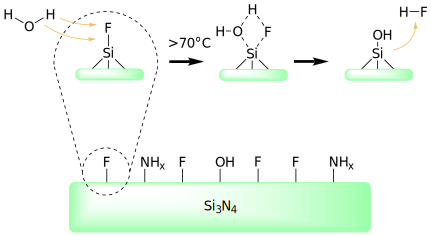
\includegraphics[width=1\linewidth]{Ressources/Chemistry/SiN}
	\capption{Proposed modification of \gls{sin} with \gls{hf}}{}
	\label{fig:chem:func:sin}
\end{wrapfigure}
One of the used substrates in this work is \gls{sin} as passivation layer above magnetic sensors as it has a significant better diffusion barrier against water or sodium ions and is chemically very inert. \cite{lit:chem:sin:surface} However, due to its complex crystal structure it is also difficult to modify by common chemicals and the exact surface composition still subject to scientific discussion. \cite{lit:chem:sin:etchingcontrol} Apart from cleaning the surface with piranha, few other modification methods have been reported, but only one suitable for the direct generation of \gls{hydroxyl} groups.

There, as depicted in \ref{fig:chem:func:sin}, the reaction \ch{Si-OH + HF <-> Si-F + H2O} takes place reversibly due to the coincidence that \ch{Si-O} and \ch{O-H} as well as \ch{Si-F} and \ch{H-F} bonds have similar binding energies and hence the forward and reverse reactions a low activation energy. After Le Chatelier's principle, a depletion of \gls{hf} in the bulk leads then to an increase in surficial hydroxyl groups. \cite{lit:chem:sin:SiFSiOH} In further works, it has been determined that an oxidation with a similar protocol based on aequous \gls{hf} yields a variable \gls{siloxane} coverage with \SI{37(17)}{\percent} of a monolayer, which nevertheless can be used for stable, covalent attachment of silanes.  Nominally the same surface coverages of silicon oxide and nitride surfaces could be achieved by ethoxy- and chlorosilanization. \cite{lit:chem:sin:surfacEtchingandMod} As shown by \citep{lit:chem:sin:silane}, the subsequent surfaces exhibit beneficial biological properties and can be modified by further standard procedures.


\subsubsection{Oxygen Plasma}
Apart from wet chemistry methods, the exposure of a surface to oxygen plasma yields \gls{hydroxyl} groups as well. In a plasma chamber, a low-pressure gas is irradiated by \si{\kilo\hertz} to \si{\mega\hertz} waves to excite and ionize its atoms. In consequence, the UV-radiation emitted by the gas can photolyse typical organic bonds and remove surface contaminations. Additionally, reactive oxygen species such as \ce{O2+}, \ce{O2-}, \ce{O3} or \ce{O} either oxidize the surface as well or bind dissociated components with low vapor pressure. During an evacuation in the process, these molecules are removed from the chamber intrinsically. \cite{lit:chem:plasma}  

\subsection{Silane Chemistry}

By the use of silane chemistry a surface is rendered organofunctional with alkoxysilane molecules. Since glass, silicon, alumina, titania, and quartz surfaces, as well as other metal oxide interfaces, are rich in hydroxyl groups, silanes are particularly useful for modifying these materials. \cite{lit:chem:silanizingGlass}\\The general formula for a silane coupling agent (Fig. \ref{fig:chem:trialkoxysilane}) typically
shows the two classes of functionality. X is a hydrolyzable
group typically alkoxy, acyloxy, halogen or amine.
\\\begin{wrapfigure}[9]{r}{.25\linewidth}
	\vspace{-0.7\baselineskip}
	\centering
	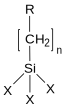
\includegraphics{Ressources/Chemistry/Trialkoxysilan}
	\capption{Trialkoxysilane}{Structure of a typical trialkoxysilane, X: hydrolyzable group, R: non-hydrolyzable organic radical, n: methylene chain-length}
	\label{fig:chem:trialkoxysilane}
\end{wrapfigure} 
Following hydrolysis, a reactive \gls{silanol} group is formed, which can condense with other silanol groups to form \gls{siloxane} linkages. 
(Fig. \ref{fig:chem:APTES}) Stable condensation products are also formed with
other oxides such as those of aluminum, zirconium, tin,
titanium, and nickel. Less stable bonds are formed with
oxides of boron, iron, and carbon, whereas alkali metal oxides and
carbonates do not form stable bonds with \glspl{siloxane} at all. The R group (Fig. \ref{fig:chem:trialkoxysilane}) is a nonhydrolyzable organic radical that may posses a functionality that imparts desired characteristics. One of the more common silanes is \gls{aptes}, where the X group consists of an \gls{ethoxy} group, the organic rest R is substituted by an \gls{amine} and the 3 \gls{methylene} groups alter \textit{n} to 3. \cite{lit:chem:GELEST} 
\begin{figure}[h]
	\centering
	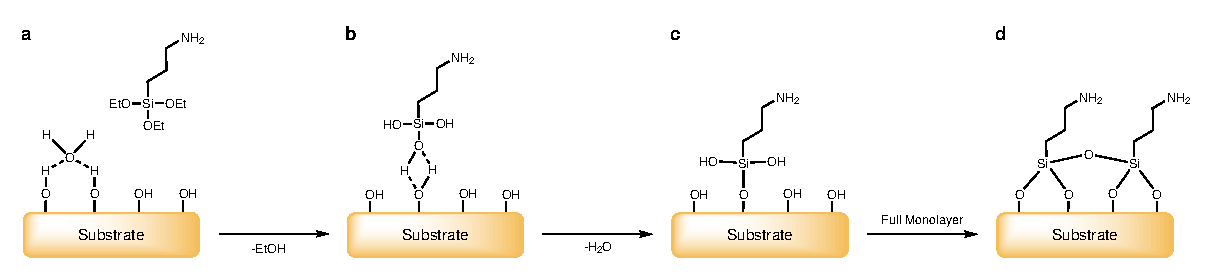
\includegraphics[width=1\linewidth]{./Ressources/Chemistry/APTES.eps}
	\capption{APTES Modifcation of an oxidized surface}{\textbf{a} Before the condensation reaction, the oxidized surface forms hydrogen bonds with water molecules. The silane molecules are in the bulk solution. \textbf{b} The hydrolyzed \gls{silanol} group adsorbs onto the surface and forms hydrogen bridges with it. \textbf{c} In a condensation reaction, under the loss of water, a covalent bond to the surface forms. \textbf{d} After the \gls{sam} assembly the surface is saturated with a covalent-bound, crosslinked silane film. \cite{lit:chem:aptes:SilaneReaction}}
	\label{fig:chem:APTES}
\end{figure}

The final result of reacting an organosilane with a substrate ranges from altering the wetting or adhesion characteristics of the substrate, utilizing the substrate to catalyze chemical transformation at the heterogeneous interface, ordering the interfacial region, and modifying its partition characteristics. Significantly, it includes the ability to effect a covalent bond between organic and inorganic materials. Especially in optical or biological sensors, silane modifications open a broad range of applications. 

However, the silanization reactions bear a few drawbacks which are often neglected. For instance, silane chemistry is strongly temperature and pH-dependent. \cite{lit:chem:silaizationTemp,lit:chem:silanizationParameters} Further, in a process to build \glspl{sam} out of \gls{aptes}, the reaction has to be catalyzed by water. But already small changes in the water content cause dramatic deviations in layer thickness. \cite{lit:chem:sin:selectivemod} Additionally, silanes can crosslink to themselves through possible side reactions. (Fig. \ref{fig:chem:APTES} D) \cite{lit:chem:aptes:Crosslink}



\subsection{Carbodiimide Crosslinker Chemistry}
The in previous manner produced \gls{amine}-terminated films by \gls{aptes} form the basis of many reactions and open the possibility to various applications, such as the direct attachment of biofunctional molecules by carbodiimide crosslinking chemistry.\cite{lit:bio:BioconjugateTechniques} Here, \gls{carboxyl} groups are modified by \gls{edc} and \gls{nhs} to form a stable secondary \gls{amide} bond with any primary \gls{amine}.

\begin{figure}[htb!]
	\centering
	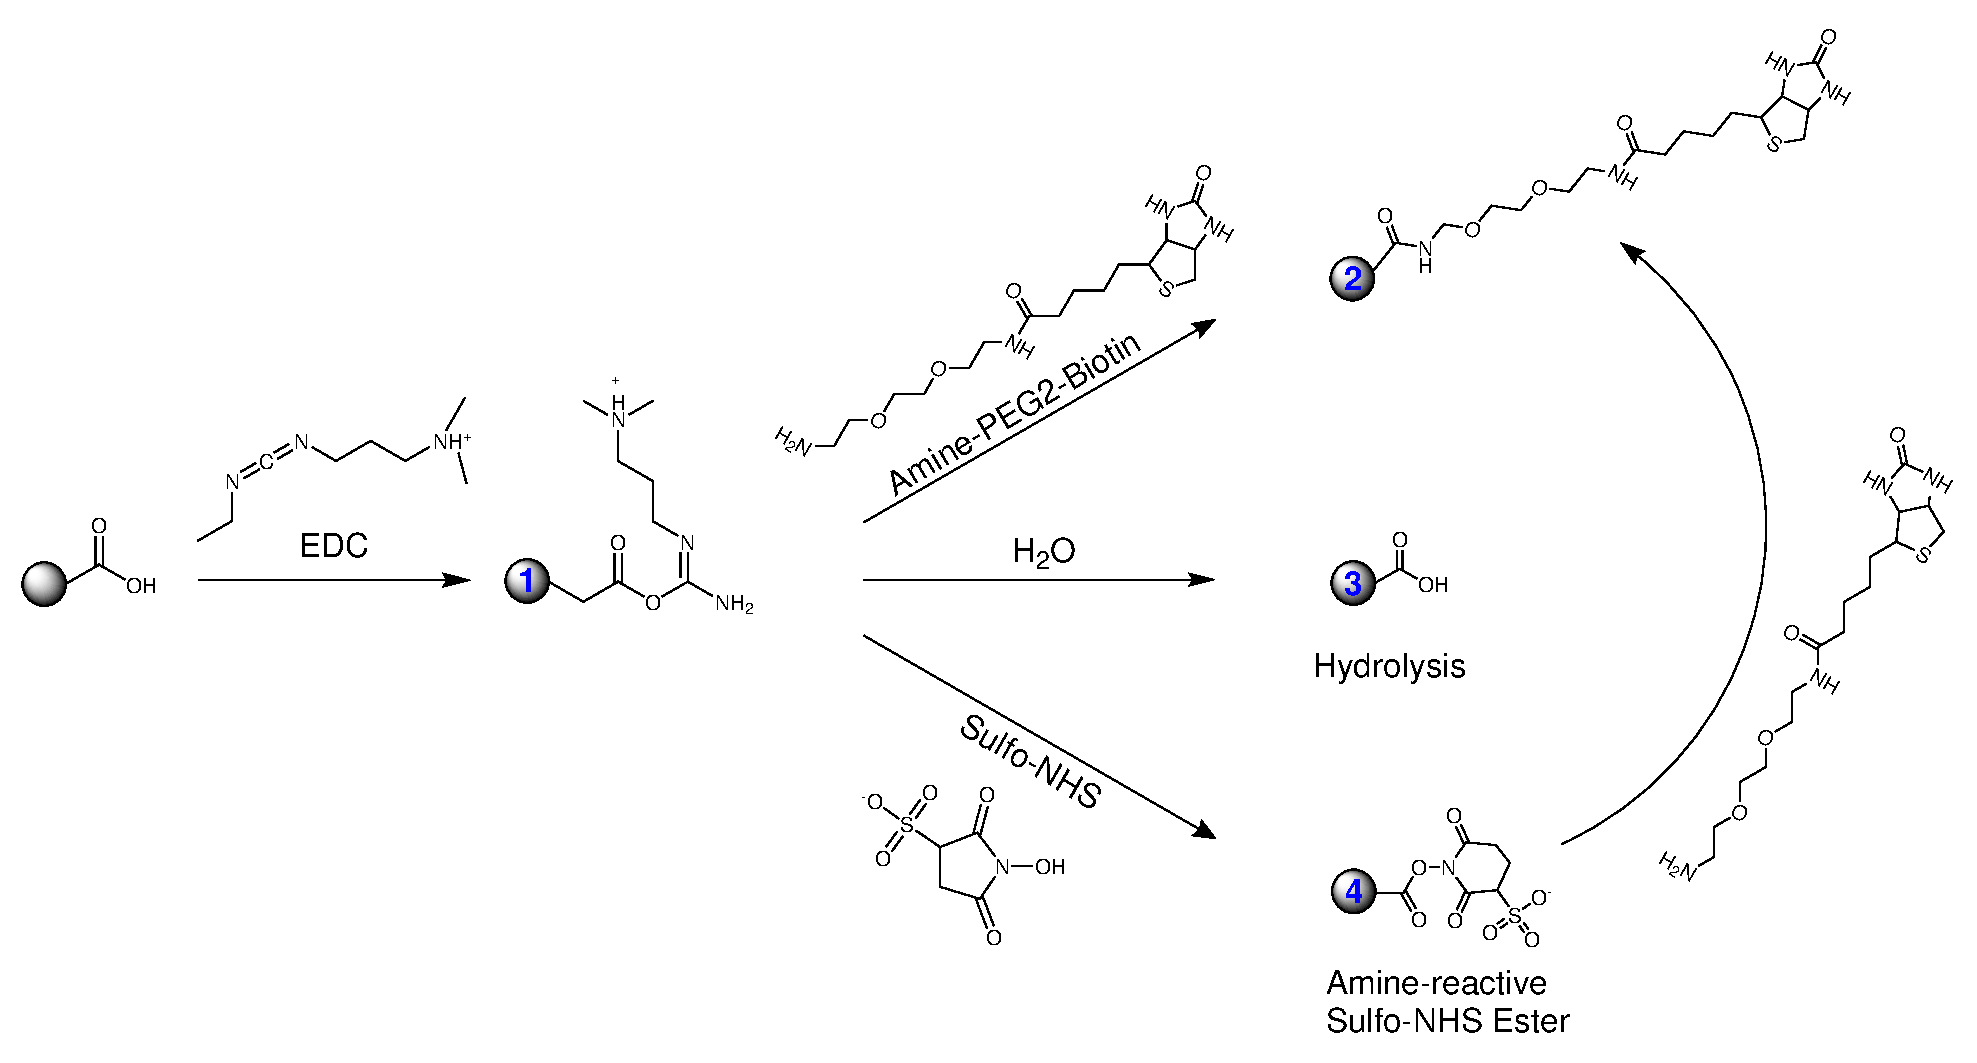
\includegraphics[width=\linewidth]{./Ressources/Chemistry/EDC-NHS.eps}
	\capption{Carboxyl bead modification with EDC/NHS}{The carboxy groups bead are activated with \gls{edc} to an active O-acylisourea intermediate. This can then either be nucleophilicly attacked by a primary amine of the amine-PEG$_2$-biotin reactant or - due to its instability - hydrolzed back to a regenerated carboxyl surface. A present NHS-ester can also displace the O-acylisourea to form a considerably more stable intermediate which then itself reacts with any primary amine.}
	\label{fig:chem:COOH-EDC-NHS}
\end{figure}
\clearpage
The general reaction mechanism is depicted in Fig. \ref{fig:chem:COOH-EDC-NHS} for the example of a microbead surface, but it can equivalently be applied to any other modified surface or molecule. The initial \gls{carboxyl} group is esterified by \gls{edc} to an active o-acylisourea intermediate and leaves rapidly upon nucleophilic attack of an amine with release of an iso-urea byproduct. A zero-length amide linkage is formed. (Fig. \ref{fig:chem:COOH-EDC-NHS}, 1->4) Sulfhydryl and hydroxyl groups also will react with such active esters, but the products of such reactions, thioesters and esters, are relatively unstable compared to an \gls{amide} bond. (Fig. \ref{fig:chem:COOH-EDC-NHS}, 1)\newline
However, this reactive complex is slow to react with amines and can hydrolyze in aqueous solutions, having a rate constant measured in seconds. If the target amine does not find the active \gls{carboxyl} before it hydrolyzes (Fig. \ref{fig:chem:COOH-EDC-NHS}, 3), the desired coupling cannot occur. This is especially a problem when the target molecule is in low concentration compared to water, as in the case of protein molecules. Notwithstanding, forming a \gls{nhs} ester intermediate from the reaction of the \gls{hydroxyl} group on NHS
with the \gls{edc} active-ester complex increases the resultant amide bond formation remarkably. (Fig. \ref{fig:chem:COOH-EDC-NHS}, 3->4) \cite{lit:chem:nhs2}

Another critical point in carbodiimide chemistry is the solubility of the compounds. \gls{edc}, \gls{nhs} and \gls{snhs} are soluble in aqueous and organic solvents. Nevertheless, activation  with  non-sulfonate \gls{nhs} decreases water-solubility of the modified carboxylate molecule, while activation with \gls{snhs} preserves or increases its water-solubility by virtue of the charged sulfonate group. \cite{lit:chem:snhs}

\clearpage

\subsection{Microscopic Particle Surface Physics}

\subsection{The Biotin-Avidin-System}


\section{Magnetoresistive Sensing}
Short intro over MRCyte
Foto of setup with arrows to necessary parts
Microscope
Stages
PEEK holder
Helmholtz coils
Kepco
MFLI
DAQ



\subsection{Sensing Principle}

Loss because of reduced velocity and magnetic drag

Different produced GMR stacks
Wheatstone Bridge setup
Magnet alignment


\chapter{Materials and Methods}

\section{Magnetic Sensor Device} 

\subsection{Assembly of Sensor}
\label{sec:meth:sensor}
The fabrication of a microfluidic device on various substrates and layouts consists of two parallelizable workflows. First, the \gls{gmr}-sensor chip (Sensitec GmbH, Germany) is assembled into a custom designed PCB (PIU-PRINTEX GmbH, Austria) by double sided adhesive tape and a square glass slide (\SI{25}{\milli\meter}x\SI{25}{\milli\meter}, Thermo Fisher Scientific, USA) at the bottom. The device is electrically contacted via wedge wire bonding (HB10, TPT Wire Bonder GmbH \& Co KG, Germany) with an aluminium wire ($\varnothing$ \SI{25}{\micro\meter}). The optimal parameters are listed in table \ref{tab:params_wirebonding}. 
\begin{table}[htb]
	\centering
\begin{tabularx}{.5\linewidth}{ccc}
	\toprule[1pt]
	Parameters & Bond 1 & Bond 2 \\
	\midrule
	Ultrasonic Power & 250 & 300 \\
	Time / ms & 200 & 200 \\
	Force / mN & 250 & 300 \\
	\bottomrule[1.2pt]
\end{tabularx}
\caption{Wirebonding Parameters}
\label{tab:params_wirebonding}
\end{table}
However, crucial for successful wire bonding is the optimal hole shape in the welding tool. Therefore, it was cleaned when bonds failed for no obvious reason by removing the gold wire and dipping the tip of the wedge into \gls{ipa}. Then, \textit{Test USG} was alternated for several seconds in multiple iterations. Afterwards, the wedge was blown dry from all sides with pressurized air and the wire was loaded back into the tool.
After wire bonding, the manufactured sensors were placed in a wafer shipper box and stored in a dust free environment for later use.
\subsection{Design and Fabrication of Microfluidics}
In the second workflow, a microfluidic channel was manufactured via photo- and softlithography and bonded to the magnetic sensors from \ref{sec:meth:sensor}.
\subsubsection{Development of Layout}
Layouts for the microfluidic channels were designed after common practices via AutoCAD (2020, Autodesk Inc., USA). The design was joined to single, closed polylines after the design finish. The files were also scanned for double lines or arcs as these cause failures in the downstream processing. The design was then exported to a compatibility \textit{*.dxf} version with a single layer of polylines.
\subsubsection{Patterning of Photoresist}
\SI{3}{\inch} (100) silicon wafers (Si-Mat - Silicon Materials e.K., Germany) were dehumidified in a drying oven (UN30, Memmert GmbH + Co.KG, Germany) for \SI{2}{\hour} at \SIrange{150}{180}{\degreeCelsius}. Then, immediately after they reached room temperature, they were placed centered inside a wafer spinner (WS-650-23B, Laurell Technologies Corp., USA). For the desired layer thicknesses \SIrange{2}{3}{\milli\liter} SU8-30XX (Kayaku Advanced Materials Inc., USA) were poured carefully onto the center of the wafer and the following program was carried out:
\begin{enumerate}[noitemsep]
\item \SI{500}{\rpm} for \SI{10}{s} at \SI{100}{\rpm\per\second}
\item \SI{3000}{\rpm} for \SI{30}{s} at \SI{300}{\rpm\per\second}
\item Ramp down at \SI{300}{\rpm\per\second}
\end{enumerate}
Upon finish, the wafer was gripped outermost with wafer tweezers and soft-baked on a hot plate (Supernuova+, Thermo Fisher Scientific, USA) for \SI{5}{\minute} at \SI{65}{\degreeCelsius} and at least \SI{10}{\minute} at \SI{90}{\degreeCelsius}. The optimal duration was determined if the gently touched resist did not stick to the tweezers. To prevent cracks in the resist caused by a fast temperature change, the wafer was cooled on the hotplate to room temperature. Such processed wafers were stored for a maximum of \SI{4}{weeks} in a light-tight storage box.\\
To pattern the resist, the i-Line of a laser lithograph (Dilase 250, Klo\'{e} SA, France) was used. In preparation of the writing, a layout \textit{*.dxf}-file  was imported to the program ``Kloe Design'' (Klo\'{e} SA, France), converted to contours and subsequently to polygons. For the filling a spot-size equivalent to the minimal structure resolution (as measured in \citet{lit:tech:rojda2020}) and an overlap of at least \SI{50}{\percent} was chosen. Departure and End Stabilization were chosen to \SI{.5}{\milli\meter} in a horizontal infill pattern. Also, flags for \textit{auto-reverse mode}, \textit{apply multiple trigger}, and \textit{detect partial/full overlap} have been set.  The writing trajectories were displayed for a last control before the export to ensure only closed contours. Finally the contour and filling were exported into separate files.\\
Both files were loaded in this order into the program ``Dilase 250'' (Klo\'{e} SA, France. Also the preprocessed wafer was placed inside the laser writer and attached to the vacuumed stage. With the integrated camera the global zero was set to the wafer center by finding the horizontal or vertical edges and adding/subtracting the radius of the wafer (\SI{1.5}{\inch} $\approx\ \varnothing $  \SI{38.1}{\milli\meter}). The focus point was set to the top of the resist and subsequently moved \SI{.07}{\milli\meter} relative down for thick layers. Then the program was initiated with \SI{100}{\percent} laser modulation and \SIrange{20}{40}{\milli\meter\per\second} writing velocity.

\subsubsection{Soft Lithography}
The fabricated wafer was placed the center of a \SI{90}{\centi\meter} petri dish. A \gls{pdms} mold was created by vigorous mixing of the pre-polymer base with its curing agent (Sylgard 184, Dow Silicones Corp., USA) in a ratio of 10:1 (w/w). For \SI{3}{\inch} wafers, thin channels were casted from \SI{15}{\gram}, channels with standard thickness from \SI{20}{\gram} \gls{pdms} in the petri dish. Gas bubbles were removed from the mixture in a desiccator for \SI{20}{\minute} at \SI{2}{\hecto\pascal}, and the \gls{pdms} was cured in an oven (UN30, Memmert GmbH + Co.KG, Germany) for \SI{1}{\hour} at \SI{60}{\degreeCelsius}. After curing, the \gls{pdms} mold was released from the petri dish carefully, taken off the wafer and stored in a clean petri dish upon further processing.  

\subsubsection{Bonding of Microfluidics}
Under a laminar flow hood, crosslinked molds were cut into the single fluidics with a razor blade. Holes for in- and outlet were added with a biopsy puncher ($\varnothing $ \SI{0.5}{\milli\meter}, Welltech Labs, Taiwan). The substrates and channels were sonicated in acetone and \gls{dih2o} for \SI{5}{\minute}, and dried with filtered \gls{n2} completely. For the bonding of \gls{pdms} to various substrates different protocols have been established:

\subsubsection{PDMS Glueing}
\label{sec:meth:bond:glue}
Here, a micron-height layer of uncured \gls{pdms} was used as an adhesive layer between the channel and the underlying substrate. Approx. \SI{3}{\milli\liter} were poured onto a \SI{3}{\inch} wafer and spun down for \SI{5}{\minute} at \SI{6000}{\per\minute}. The microchannel was placed on the substrate by visual control of a stereo microscope (SMZ800, Nikon GmbH, Germany) with 8-fold magnification. Subsequently, the bonding process could be finished by a \SI{1}{\hour} bake at \SI{60}{\degreeCelsius} or over-night at room temperature.
\subsubsection{Plasma Bonding}
\label{sec:meth:bond:plasma}
The respective parts were activated by the exposure to a controlled \gls{o2}-plasma. Bringing the activated surfaces in contact immediately triggers the formation of covalent bonds. First, the acetone-wiped substrates and the microchannels were centered inside the plasma cleaner (Zepto, Diener electronic GmbH \& Co KG, Germany). Second, vacuum was applied to a final pressure <\SI{0.2}{\hecto\pascal}. Third, the chamber was flushed with pure \gls{o2} until a chamber pressure from \SIrange{0.6}{0.8}{\hecto\pascal} had been stabilized. Fourth, the plasma process was executed with \SI{30}{\watt} (Power-Potentiometer: 100) for \SIrange{45}{60}{\second} (Time-Potentiometer: 15-20). Upon finish, the chamber was flushed for \SI{5}{\second} and ventilated. Immediately after, the corresponding workpieces were brought into contact and pressed together gently. To ensure a durable bond, the assembled structures were baked for \SI{1}{\hour} at \SI{60}{\degreeCelsius}.
\subsubsection{Reversible Bonding}
To bond the microfluidic to a substrate reversibly and without residues, the channel was brought into contact with the bottom part without any adhesinon agent. For low-pressure as well as vacuum driven flows, this method is preferrable due to its time and work efficiency.
\subsection{Peripheral Components and Optical Readout}
Each sensor chip was characterized by the hysteresis steepness (equivalent to the sensitivity) and the zero-crossing at half-maximum in a customized setup. Therefore, the underlying 32 x 27 x \SI{5}{\milli\meter} NeFeB magnet (NE3227, IBS Magnet e.K., Germany) was adjusted on micromanipulator tables (PT, Thorlabs GmbH, Germany) in three axes to optimize both parameters. Afterwards, teflon-tubing (ID \SI{0.5}{\milli\meter}, RCT Reichelt Chemietechnik GmbH + Co., Germany) was connected on the in- and outlet of the microfluidic. A dispensing tip (OD $\varnothing$ \SI{0.42}{\milli\meter}, Nordson Deutschland GmbH, Germany) was connected to the inlet tubing. Initially a \SI{1}{\milli\liter} syringe (ID \SI{4.72}{\milli\meter}, Terumo GmbH, Germany) was connected with \gls{dih2o} or \gls{pbs} and flushed with \SIrange{100}{200}{\micro\liter\per\minute} by a syringe pump (Fusion 4000, Chemyx Inc., USA).
\begin{figure}
	\centering
	\centering
	\subfloat{
		\subfigimg[height=150pt]{a}{Ressources/ResultPlots/Hysteresis_D}
		\phantomsubcaption
		\label{fig:meth:Hyst:mr}	
	} \hfill
	\addtocounter{subfigure}{-1}
	\subfloat{
		\subfigimg[height=150pt]{b}{Ressources/ResultPlots/Sensitivity_D}	
		\phantomsubcaption
		\label{fig:meth:Hyst:sens}
	}
	\capption{Hysteresis Calibration of the \gls{gmr}-Sensor}{Sensitivity Optimization of the \gls{gmr} senor via alternating hysteresis measurements and permanent magnet adjustment. (\textbf{a}) Optimal sensitivity is reached when the zero-crossing is centered around the zero-field and the linear section has the maximum steepness.(\bluedash) Upon dislocating the free layer in one direction, the magnetic field strength increases linearly towards saturation.(\orangeline) Afterwars, the magnetization moves on the hysteresis loop. The total \gls{mr} is calculated from the vertical distance between the saturation points. (\greenline) (\blackline) (\textbf{b}) In order to determine the steepness in the linear section, the hysteresis from the left side is differentiated. Actual sensitivity (\bluedash) is measured by the mean of all curves in the zero field. The initial magnetization curve is omitted from this measurement.(\orangeline) }	
	\label{fig:meth:Hyst}
\end{figure}
\subsubsection{Hysteresis Alignment}
Prior to the cell counting experiments \gls{gmr} sensors were characterized.  Adjustment of the position of the permanent magnet relative to the sensors was performed via hysteresis measurement.(\cref{fig:meth:Hyst})  Therefore, an in-plane field was applied to the sensor was imposed by two Helmholtz coils ($L_s$ = \SI{167}{\milli\henry}, d = \SI{150}{\milli\meter}, Dr. Brockhaus Messtechnik GmbH \& Co. KG, Germany) generating \SI{7.8}{\milli\tesla\per\ampere} orthogonal to the easy axis of the \gls{gmr} which were driven by a voltage-controlled current source (BOP 50-8M, Kepco Inc., USA) with $\pm$ \SI{2}{\ampere} at a \gls{el:vpp} of \SI{20}{\volt}. The control voltage was supplied by LabView (2018, 32-bit, National Instruments Corp., USA) supplied by a digital I/O card (USB-6351, National Instruments Corp., USA) in the range of \SIrange{-10}{10}{\volt}.
The resulting sensor signal was fed into the current input of a lock-in amplifier (\gls{mfli}, \SI{5}{\mega\hertz}, Zurich Instruments AG, Switzerland) with a filter constant of \SI{1}{\milli\second}.
Re-digitization and processing was carried out by the same digital I/O card and LabView program as for the input control.

In effect, the sensitivity was computed from the hysteresis' steepness in the magnetic zero-field. Hereby, the very first hysteresis loop was omitted for further calculations because it contains the initial magnetization curve.(\cref{fig:meth:Hyst:mr}) By differentiating the hysteresis (\cref{fig:meth:Hyst:sens}), the maximum \gls{mr} per unit magnetic field could be computed from the numeric maximum in $x = 0$. During the course of the thesis, it resulted typically in \SI{1.2 +- 0.2}{\percent\per\milli\tesla}.\footnote{It should be noted that this value depends on the normalization method. Typically, the sensitivity is measured from the hysteresis which is corrected for their minimum value per definitonem of the \gls{gmr} effect. In a real measurement, at an external actuation displaces the free layer from the magnetic zero-field. Therefore, a measurement would have to be corrected by the zero-field value. However, this causes a relatively small error which is solely relevant for quantitative calculations.} From this, the bridge sensitivity could be also expressed in unit of \si{\ohm\per\milli\tesla}. With a typical \gls{gmr} resistance of \SI{300 +- 50}{\ohm} and a supply of \gls{el:vpp} = \SI{200}{\milli\volt}, the typical voltage drop results in \SI{840 +- 130}{\micro\volt\per\milli\tesla}.\footnote{Output Voltage of one bridge branch: $V_{out} = \frac{R_{sig}}{R_{const}+R_{sig}}\cdot \frac{V_{pp}}{2\sqrt{2}}$}
\subsubsection{Single GMR} \label{sec:meth:singleGMR}
The change in resistivity over one whole Wheatstone bridge was measured with the \gls{mfli} under a supply \gls{el:vp} of \SIrange{100}{800}{\milli\volt}. The reference frequency was chosen randomly in a range of \SI{100(25)}{\kHz} such that any harmonics were avoided. The measured differential bridge balance was then demodulated and filtered with a time constant of \SI{299.7}{\micro\second} by a third order low-pass filter and amplified by the factor \num{10000}. Subsequently, the processed signal was sampled at \SI{53.2}{\kilo\siemens\per\second} from the \gls{mfli} and subsequently from an 16-bit analog-to-digital converter (USB-6351, National Instruments Corp., USA) with input range of \SI{+-10}{\volt} and  \SI{10}{\kilo\siemens\per\second}.\newline
During sensor operation, a 20x microscope image (DM2500M, Leica Microsystems GmbH, Germany) was captured by a CCD-camera (Grasshopper3, FLIR Systems Inc., USA) and displayed in real-time to control the experiment.
\subsubsection{Dual GMR}
\label{sec:meth:dualGMR}
For the measurement of two GMR-sensors simultaneously, the setup from \ref{sec:meth:singleGMR} was duplicated in two different manners. However, the exact same settings in the device control software were crucial for successful measurements.  In a first approach, the supply cable of one \gls{mfli} was split and fed into both sensors, while the bridge balance was evaluated by the same and an additional lock-in, both with the exact same settings. Consequently, the ground pin of the one sensor was the reference also for the other sensor and one ground pin was therefore left floating. This method posed the least cable length and therefore noise, but was also prone to cross-talking between the used BNC-cables respectively -connectors.\\
Second, two \gls{mfli}'s were driven in a master-slave clock synchronization by the Multi-Device Sync function. Therefore, the \textit{trigger out} and \textit{clock out} ports on the backside of the master were connected to the slave's \textit{trigger in} and \textit{clock in} ports. Additionally, the \textit{trigger out} was split by a T-connector piece in order to feed it also back into the master's \textit{trigger in} port.\\
In both cases, the output of both lock-ins was directed to their respective \textit{AUX 1} ports and connected to another LabView program by the previously mentioned DAQ-card.
\subsubsection{Differential Sensor Setup}
In some experiments, two PCBs were stacked with nylon spacers (D01482, DURATOOL Corp, Taiwan) with various lengths \SIlist{3;5;8}{\milli\meter} between their edges above the permanent magnet. Before the stacking, outlet tubing of the upper chip was connected to the inlet of the lower chip with the least dead volume possible.\\ Then, immediately before assembly, the channels were flushed with buffer and were inspected to confirm the absence of gas-bubbles. After the final assembly, the hysteresis was adjusted for both sensors on various bridges consecutively. Measurements were performed as described in \ref{sec:meth:singleGMR} with two completely independent lock-in amplifiers.
\subsubsection{GMR Data Analysis} \label{sec:meth:gmrDataAnalysis}
Subsequent data analysis of the acquired streams from both two and one sensor measurements were modified by a custom labview VI to cut the first sample of the stream which was mandatory for the next step. Next, the characteristic signal patterns were detected in the continuous stream by the \textit{GMR\_Tool\_227} by a rolling-mean thresholding method. The resulting \textit{*\_ana.csv} files were then processed by a custom Matlab script, which in turn computed averages and simple parameters of a single detected signal or whole measured, p.e. the total volume or the signal count therein. The Matlab script saved any analyzed data also in the \textit{*.csv} format.
\section{Magnetic Beadometry}
Magnetic beads were measured in various manners. First, beads were pumped over substrates under microscope control (DM6, Leica Microsystems GmbH, Germany) with simultaneous image acquisition for count (LAS X, Leica Microsystems GmbH, Germany) and trajectory analyses (ImageJ Fiji, \cite{lit:chem:Fiji}). Second, beads were measured in buffer or diluted whole blood samples to determine their concentration in the magnetic flow cytometer. The previous measurements were then adapted to functionalized surfaces in order to detect a difference in concentration. In all experiments, teflon tubing (ID \SI{0.5}{\milli\meter}, RCT Reichelt Chemietechnik GmbH + Co., Germany), dispensing tips (OD \SI{0.42}{\milli\meter}, Nordson GmbH, Germany), \SI{1}{\milli\liter} syringes (ID \SI{4.78}{\milli\meter}, Terumo GmbH, Germany), a syringe pump (Fusion 4000, Chemyx Inc., USA) and a microfluidic channel with dimension \SI{700}{\micro\meter} x \SI{150}{\micro\meter} (width x height) were used.
\subsection{Optical Particle Tracking}
In order to track particles in microscopy images pictures were processed in Fiji (ImageJ, \cite{lit:chem:Fiji}). Subsequently, they were either counted manually in a measured volume or tracked by the TrackMate Plugin \cite{trackmate}. \\
Initially, the microscope pictures were imported with the \textit{BioFormats Importer} as tiff-stacks. The region of interest was selected with a polygon and cropped. Then, the stack was converted to 8-bit and thresholded by the \textit{Yen dark} algorithm. After an inverting the images, a slice with no visible beads was subtracted from the stack.  The result was used for manual counting.\\
For the tracking, the \textit{LoG-Detector} with a \textit{blob diameter} of \SI{8}{\micro\meter} has been used with a threshold of \num{2.0}. Additional flags were set for \textit{use median filter}, \textit{subpixel localization} and \textit{hyperstack}. The resulting particle detections were visualized by their respective \gls{snr}. Subsequently, the \textit{linear motion LAP tracker} was initialized with a motion radius of \SI{60}{\micro\meter} and a search radius of \SI{60}{\micro\meter} through the maximum frame number. 
\subsection{Absolute Concentration Measurement}
\label{sec:meth:conc}
Before every measurement, the initial bead concentration was determined meticulously in a Neubauer Improved counting chamber or by flow cytometry and adjusted between \SIrange{1}{10}{\per\micro\liter} in \gls{pbst}. Then, after the sensor was calibrated accordingly in the single or dual \gls{gmr}-setup (\cref{sec:meth:singleGMR,sec:meth:dualGMR}), beads were pumped at a fixed flow rate of \SI{80}{\micro\liter\per\minute} and \SI{30}{\micro\liter\per\minute} through a channel with \SI{150}{\micro\meter} or \SI{50}{\micro\meter} height, accordingly. Either the previously mentioned plastic syringe or a \SI{1}{\milli\liter} glass syringe (1001 TLL, Hamilton Bonaduz AG, Switzerland) was utilized in a syringe system for these experiments. The duration to attain statistical significance was specified by a minimal volume \SI{300}{\micro\liter} or a detection of at least \num{300} particles. Between samples, the whole system was flushed with \gls{pbst} at flow rates greater than \SI{150}{\micro\liter\per\minute} or \SI{60}{\micro\liter\per\minute}, respectively to \SI{150}{\micro\meter}/\SI{50}{\micro\meter} channel heights. Afterwards, signal streams were analyzed according to the procedure in \cref{sec:meth:gmrDataAnalysis}.
\subsection{Whole Blood Bead Spiking}
For measurements in whole blood samples,\SI{6}{\milli\liter} blood were drawn from test subjects in \SI{7.5}{\milli\liter}, \gls{edta}-containing vials (S-Monovette Hämatologie, Sarstedt AG \& Co. KG, Germany). Beads with precise concentrations were prepared according to \cref{sec:meth:conc} in \gls{pbs}. Then, several dilutions of whole blood were created from the particle solutions and mixed carefully with a \SI{1}{\milli\liter} micro-pipette or by inversion. The samples were subsequently measured at a fixed flow rate of \SI{40}{\micro\liter\per\minute} in a \SI{150}{\micro\meter} channel. In between samples, the channel has been flushed with \gls{macs} buffer at high flow rates as in \cref{sec:meth:conc}. The best measurements arose from S48 chips with broad, \SI{200}{\nano\meter}-high nickel-iron structures.
\subsection{Bead Capture Assay}
As prequisite for the bead capture assay, the different self-biotinylated particles (\cref{sec:meth:particle}) were diluted as for the concentration measurement in \cref{sec:meth:conc}.  Further, a GMR sensor was fabricated, loaded unspecifically with \SI{1}{\milli\gram\per\milli\liter} neutravidin, hysteresis aligned and connected in the single GMR setup (see \ref{sec:meth:singleGMR}). As first step, the bead adhesion was determined by finding the minimal flow rate at which non-biotinylated beads were still rolling freely and at second, by finding the maximal flow rate at which biotinylated beads were still notably captured, both by microscope oberservation and sensor signal analysis. The average flow rate of these two was consequently held constant over all experiments. Subsequently, beads with different surface coverages of biotin were pumped alternatingly through the channel and over the sensor. The generated data was analyzed after the standard protocol in \ref{sec:meth:gmrDataAnalysis}.
\section{Surface Bio-Functionalization}
\subsection{Surface Activation}
\label{sec:meth:surfActiv}
To functionalize any silicon containing surface with \ch{Si\bond{sb}OH} groups which the utilized silane could interact with, multiple surface activation pathways were explored. First, substrates were cleaned in \gls{hcl}:\gls{meoh} and \gls{h2so4} before they were immersed in boiling water. Second, surface silanol groups were achieved by piranha immersion. Third a \gls{hf} dip and fourth a oxygen plasma treatment was tested.\\
For all methods, the following reagents were used: \gls{dih2o} (\SI{0,054}{\micro\siemens}, Merck MilliQ)), acetone (\SI{>99,9}{\percent}, VWR International LLC, Germany), \gls{etoh} (absolute, VWR International LLC, Germany), \gls{meoh} (\SI{99.8}{\percent}, VWR International LLC, Germany), \gls{acoh} (glacial,  VWR International LLC, Germany), \gls{hcl} (\SI{37}{\percent}, Merck KGaA, Germany), \gls{h2so4} (\SIrange{95}{98}{\percent}, Merck KGaA, Germany), \gls{h2o2} (\SI{30}{\percent} (w/w), Merck KGaA, Germany), \gls{hf} (\SI{10}{\percent},  VWR International LLC, Germany),\gls{macs} (MACSQuant Running Buffer, Miltenyi Biotech, Germany), \gls{mes} (145224-94-8, Merck KGaA, Germany), \gls{edc} (25952-53-8, Merck KGaA, Germany), \gls{nhs} (6066-82-6, Merck KGaA, Germany), \gls{aptes} (919-30-2, Merck KGaA, Germany), \gls{paa} (9003-01-4, Merck KGaA, Germany), neutravidin (31050, Thermo Fisher Scientific, USA)
\subsubsection{Work Safety Remarks}
Before the work with one of the acid solutions was carried out, serveral safety measures were implemented. As any reacting acid solution becomes very hot immediately due to the exothermic reaction, every container should be placed inside a cooled water or ice bath. Additionally, the beaker as well as concentrated acid flasks should be gripped firmly by a laboratory stand to avoid a tip over. As the reactivity of chemicals is highly temperature-dependent, the solutions was processed further when they had been cooled to \SI{<=80}{\degreeCelsius}. It should be also noted that - as in every chemical reaction, but especially ones with \gls{h2so4} and \gls{hf} - the acid was always poured into the other reactant to avoid splashing and boiling.
\subsubsection{Plasma Activation}
For the plasma activation, process parameters similar to the PDMS bonding technique in \ref{sec:meth:bonding:plasma} were chosen. After inital cleaning via sonication in \gls{acoh} and \gls{dih2o} for \SI{5}{\minute} each, the substrated were dried in \gls{n2}-gas and placed inside the plasma chamber. The chamber was evacuated to a final pressure <\SI{0.2}{\hecto\pascal} and then flushed with pure \gls{o2} until a chamber pressure between \SIrange{0.6}{0.8}{\hecto\pascal} had been stabilized. Fourth, the plasma process was executed with \SI{100}{\watt} (Power-Potentiometer: \num{300}) for \SI{300}{\second} (Time-Potentiometer: \num{190}). Upon finish, the chamber was flushed for \SI{5}{\second} and ventilated.
\subsubsection{Hydrochloric-Sulfuric Acid Activation}
In order to degrease any glass or \gls{sin} surface, a protocol according to \citet{lit:chem:Dressick} was used. There, the surfaces were first sonicated in acetone and \gls{dih2o}  for \SI{5}{\minute}. Afterwards these were immersed in a 1:1 (v/v) solution of \gls{hcl}:\gls{meoh} for \SI{>30}{\minute}, rinsed with \gls{dih2o} copiously and soaked in \gls{h2so4} for \SI{>30}{\minute} as well. Then, the samples were rinsed again in \acrlong{dih2o}. To form silanol groups on the activated surface, the surfaces were finally immersed in \SI{>90}{\degreeCelsius} heated (SuperNuova+, Thermo Fisher Scientific, USA) \gls{dih2o}  for at least \SI{2}{\hour}.
\subsubsection{Piranha Activation}
In this method, activation was carried out in a 1:7 (v/v) piranha solution at \SI{70}{\degreeCelsius} for \SIrange{1}{30}{\minute}. After treatment, the samples were rinsed carefully with \gls{dih2o} three times.
\subsubsection{Hydrofluoric Acid Activation}
For \gls{hf} activation of \gls{sin}, a protocol after \citet{lit:chem:sin:surfacEtchingandMod} was reproduced. Acetone cleaned samples were immersed in \SI{1}{\percent} aequous \gls{hf} for \SI{2}{\minute} and rinsed with \gls{dih2o} extensively afterwards without letting the surface dry at any time.
\subsection{Chemical Surface Functionalization}
\label{sec:meth:surfFunc}
Chemically activated surfaces were now coupled with \gls{aptes} covalently. Therefore an aqueous silane solution was prepared from \gls{etoh} with volume fractions of \SI{5}{\percent} \gls{dih2o}, \SI{0.5}{\percent} aqueous \gls{acoh} (pH 4.5) and \SI{1}{\percent} \gls{aptes} in this order. The samples were soaked immediately after their activation in the silane solution. The reaction was carried out for \SIrange{2}{4}{\hour} at \SI{>40}{\degreeCelsius} or for \SI{1}{\hour} at \SI{70}{\degreeCelsius}. At finish, all specimens were rinsed with \gls{etoh} or sonicated for \SI{5}{\minute} in absolute \gls{etoh}.\\
Then, the amine terminated surface modification was enhanced by a carbodiimide conjugation with \gls{paa} after \citet{lit:Anti-EpCAM-PAA}. As above, a reaction consisting of \SI{1}{\milli\molar} \gls{mes} buffer (pH 6) with \SI{1}{\milli\gram\per\milli\liter} \gls{paa}, \SI{6}{\milli\molar} \gls{edc} and  \SI{3}{\milli\molar} \gls{nhs} was activated for \SI{15}{\minute} on a magnetic stirrer. Subsequently, the prepared samples were immersed in the solution for \SI{1}{\hour} on a rotation shaker. As final cleaning, the slides were rinsed or sonicated for \SI{5}{\minute} in \gls{dih2o} and stored in fresh \gls{dih2o} at \SI{4}{\degreeCelsius} up to \SI{14}{\day} upon further use.
\subsubsection{Tensiometry}
All above methods were characterized by a custom built tensiometer and the ImageJ Fiji plugin DropSnake. \cite{lit:chem:Fiji,lit:chem:surfaceTension}
In an experiment, a substrate was dried by \gls{n2} and placed in the camera focus. Subsequently, a sessile drop of \SI{1}{\micro\liter} was placed in the focus with a micro-pipette without touching the surface. The focus of the camera was adjusted meticulously to gain maximum contrast at the droplet contour and a homogeneously black droplet. Images were then acquired by an USB-microscope (toolcraft AG, Germany)
pointing in an acute angle onto a drop on the surveyed substrate, while background illumination was provided by a fiber optical illuminator (KL1500, Schott AG, Germany). The images were then cropped, rotated such that the droplet edges were aligned horizontal and converted to 8-bit grayscale. After preprocessing, the top half contour was outlined by at least 8 points inside the DropSnake plugin and the resulting contact angles were exported.
\subsection{Surface Bioconjugation}
\label{sec:meth:surfBio}
A functionalized surface from \ref{sec:meth:surfFunc}, was now bonded to a \SI{150}{\micro\meter} microfluidic channel as in \ref{sec:meth:bond:glue} and incubated for at least \SI{5}{\hour}, but mostly over night at \SI{7}{\degreeCelsius}. Upon finish, microfluidic teflon-tubing (ID $\varnothing$ \SI{0.5}{\milli\meter}, RCT Reichelt Chemietechnik GmbH + Co., Germany)  was connected to the inlet and outlet with precision tweezers. Then, the channel was equilibrated with \SIrange{100}{300}{\micro\liter} \gls{mes} buffer in a syringe (\SI{1}{\milli\liter}, Terumo GmbH, Germany) with a syringe pump (Fusion 100, Chemyx Inc., USA) with \SI{100}{\micro\liter\per\minute}. Then, \SIlist{50;100;300}{\milli\molar} of \gls{edc} and \gls{nhs} were flushed into the channel with the same flow rate after an dissociation time of \SI{10}{\minute}. The channel bottom was incubated for \SI{30}{\minute} and then washed again with \SI{100}{\micro\liter} \gls{mes} buffer. 

Subsequently, a desired protein was loaded in high concentration (Neutravidin: \SI{1}{\milli\gram\per\milli\liter}, Antibody: \SI{20}{\micro\gram\per\milli\liter},) via the tip of a \SI{1}{\milli\liter} syringe or flushed into the channel by vaccuum from a microcentrifuge tube. The functionalized channels were now incubated over night in an ice box. Before use, the channel was washed with \SI{100}{\micro\liter} \gls{pbs} with \SI{0.02}{\percent} nonionic surfactant (Tween 20, Merck KGaA, Germany) (PBST) for \SI{2}{\minute}. Any unreacted binding sites were blocked by a solution of \SI{500}{\milli\molar} ethanolamine hydrochloride (E6133, Merck KGaA, Germany) in \gls{dih2o} for 30 min. After another washing step, the functionalized channels were further used for either microscope or magnetic bead-capture experiments.

However, in some experiments focus lay on physisorption rather than on chemisorption. Therefore, after the bonding of a microfluidic channel to a non-functionalized substrate, the channel was equilibrated as mentioned before with \gls{mes} buffer (cave: without surfactant). Then it was incubated with a solution containing protein in highest concentration, p.e. \SI{1}{\milli\gram\per\milli\liter} neutravidin, at \SI{7}{\degreeCelsius} over night, while infusing and withdrawing a small volume fraction (approx. \SI{50}{\micro\liter}) continuously by a syringe pump. Upon finish, the tubing was exchanged with a drop of water a the connection and channel was flushed with \gls{pbs} carefully at \SI{50}{\micro\liter\per\minute} to avoid any gas bubbles inside the fluidic. It was stored up to \SI{10}{\day} without any notable decrease in functionality.
\subsection{Particle Functionalization}
\label{sec:meth:particle}
Micro- and nanobeads from different suppliers were used in functionalization experiments but modified after the same procedure according to their surface charge. A positive partial charge from an \gls{amine}-terminated bead and a negative partial charge from a \gls{carboxyl}-terminated bead was used to promote different electrostatic interactions with a microchannel's surface. A list of all used particles and their respective parameters are depicted in table \ref{tab:particles}.
\begin{table}[htb]
	\normalsize
	\begin{tabularx}{\linewidth}{m{17mm}m{22mm}m{8mm}m{20mm}m{20mm}m{20mm}}
		\toprule[1pt]
		Supplier & Brand Name & d (\si{\micro\meter}) & Func\-tio\-na\-li\-za\-tion & Surface Charge (\si{\micro\mol\per\gram})  & Magnetic Particle Momentum (\si{\ampere\square\meter})\\
		\midrule
		micromod & micromer & \num{8} & \gls{amine} & \num{2.0} &  0 \\		
		micromod & micromer-M & \num{8} & \gls{amine}  & \num{1.0} & \num{>1.12e-12} \\ \addlinespace
		micromod & micromer & 8 & \gls{carboxyl} & \num{2.0} &  0\\
		micromod & micromer-M & 8 & \gls{carboxyl}  & \num{1.0} & \num{>1.12e-12}\\ \addlinespace
		invitrogen & Dynabead M280 & \num{2.8} & streptavidin & \num{.65}-\num{.90} &  N.A.\\
		invitrogen & Dynabeads MyOne C1 & \num{1.05} & streptavidin & \num{>2.5} & N.A. \\
		Ocean Nanotec &  SV0050  & \num{0.05}& streptavidin & N.A. & N.A. \\
		micromod & BNF-Dextran-redF &\num{0.1} & streptavidin &\num{0.2} & \num{>1.27e-16} \\
		micromod & nanomag-D-spio & \num{0.1} & streptavidin & \num{0.02}-\num{0.04} & \num{>5.5e-17} \\
		\bottomrule[1.2pt]
	\end{tabularx}
	\caption{Properties of the used microbeads and \glspl{mnp}.}
	\label{tab:particles}
\end{table}
\subsubsection{Amine-terminated Beads} \label{sec:meth:aminebeads}
For \gls{amine} beads, \gls{nhs}-Biotin (203118, Merck KGaA, Germany) was used for a covalent attachment after the previously mentioned carbodiimide chemistry. Initially, the biotin was dissolved to a concentration of (\SI{50}{\milli\gram\per\milli\liter}) in water-free \gls{dmso} (67-68-5, Merck KGaA, Germany) and stored upon further use at \SI{-25}{\degreeCelsius}. The attachment to microbeads was titrated by the molar weight ratio of both reagents and ranged from 10-fold molar excess to a \num{10000}-fold deficit of biotin over the amine. 

In most cases, \SI{20}{\micro\liter} of micromer beads were aliquoted in several microcentrifuge tubes (\SI{1.5}{\milli\liter}, Protein LoBind, Eppendorf AG, Germany) to generate a standard curve of functionalization density later on. \gls{nhs}-Biotin was diluted to a concentration of \SI{0.5}{\milli\gram\per\milli\liter} with \gls{pbst} and vortexed. Then, beads and biotinylation reagent were mixed in the desired ratio throughly and incubated for \SI{1.75}{\hour} at \SI{8}{\degreeCelsius} in a shaker at \SI{1400}{\per\minute}.
\subsubsection{Carboxyl-terminated Beads}
The surface of \gls{carboxyl}-terminated beads was esterified by \gls{edc}-\gls{nhs} chemistry and convalently bound to amine-PEG$_\mathrm{2}$-biotin (EZ Link, Thermo Fisher Scientific Inc., USA). First, the bead buffer was exchanged to \gls{mest} with one washing step by centrifugation (as in \ref{sec:meth:aminebeads}) to a final bead concentration of \SI{5}{\milli\gram\per\milli\liter}. \SI{100}{\milli\molar} \gls{edc} in \gls{dih2o} and \SI{50}{\milli\molar} \gls{nhs} in \gls{dmso} were prepared and added to the bead solution to a final concentration of \SI{25}{\milli\molar} and \SI{12.5}{\milli\molar} each. The suspension was reacted for \SI{30}{\minute} on a shaker at \SI{1400}{\per\minute} and washed once with \gls{mest} buffer. Then,  amine-PEG$_\mathrm{2}$-biotin was added from 10-fold molar excess to a \num{10000}-fold deficit of biotin over the amine and volume adjusted. The samples were incubated on a shaker for \SI{1.75}{\hour} at \SI{8}{\degreeCelsius} in a shaker at \SI{1400}{\per\minute}.
\subsubsection{Post-Processing and Characterization of Beads}
\label{sec:meth:beadCharact}
After the incubation, the beads were washed either magnetically or via pelleting. Magnetic washing was carried out in a magnet stand, where the beads were separated for \SI{2}{\minute} and then washed 3 times with \SIrange{500}{1000}{\micro\liter} \gls{pbst}. Pellet washing was conducted three times in a centrifuge (Fresco 17, Thermo Scientific) at \SIrange{800}{1200}{x g} for \SI{10}{\minute}. The supernatant was discarded and the pellet was dissolved in \SIrange{500}{1000}{\micro\liter} \gls{pbst}. After both washing procedures, the beads were  resuspended in \SI{100}{\micro\liter} \gls{macs} or \gls{pbst} and stored at \SI{4}{\degreeCelsius}.
\begin{figure}[htb!]
	\centering 
	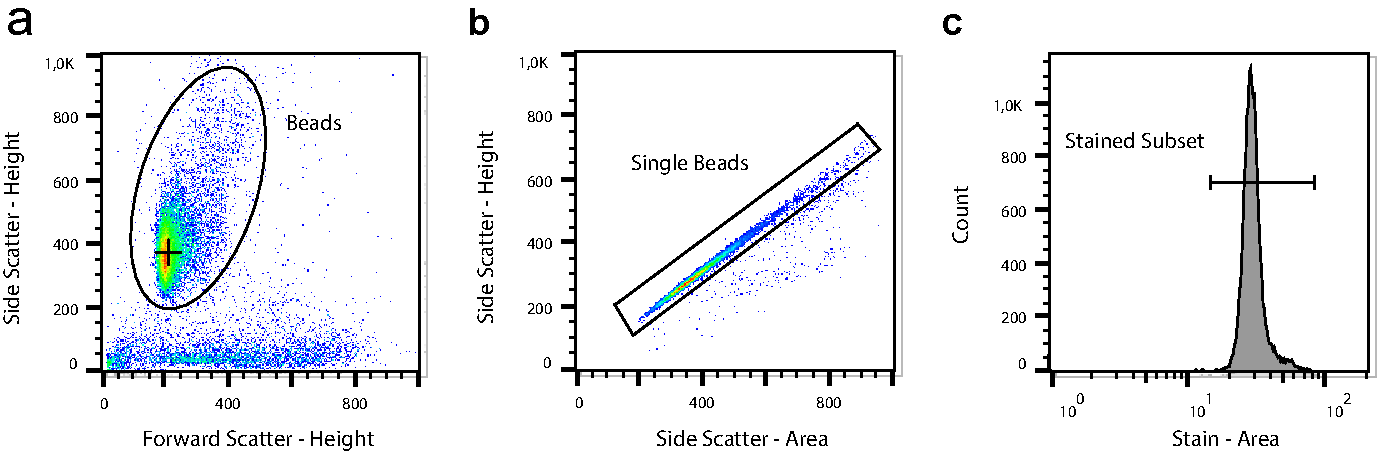
\includegraphics[width=\linewidth] {Ressources/GatingStrategy/GatingStrategy-Layout}
	\capption{Gating Strategy for Biotinylated Beads}{(\textbf{a}), In the forward-side-scatter plot, the general bead population with high side scatter is selected from the background. (\textbf{b}), Single beads are differentiated by their sphericity, their ratio of height:area in the side scatter. Points on the line through the origin are spherical. (\textbf{c}), The stained subset in the respective color is now selected and the \gls{mfi} as well as the \gls{cv} is computed.}
	\label{fig:gatingstrategy-layout}
\end{figure}

Characterization of any surface modification was done via fluorescence-flow cytometry or -microscopy. \SIrange{30000}{60000}{beads} were diluted to \SI{20}{\micro\liter} and incubated with \SI{100}{\nano\gram} streptavidin-atto488 (49937, Merck KGaA, Germany) or Anti-Biotin-PE (REA746-PE, REAfinity, Miltenyi Biotec B.V. \& Co. KG, Germany) for \SI{30}{\minute} at \SI{8}{\degreeCelsius} in a shaker. The beads were then diluted to a final volume of \SI{100}{\micro\liter}, transferred to a 96-well plate and measured in the autosampler of a flow cytometer (MACSQuant Analyzer 10, Miltenyi Biotec B.V. \& Co. KG, Germany). Following parameters were held constant over all measurements: \textit{Flow Rate:} High, \textit{Mix Sample:} Strong, \textit{Mode:} Standard, \textit{Uptake/Sample Volume:} \SI{100}{\micro\liter}. The photmultiplier voltages of forward and side scatter were lowered in most experiments by \SI{10}{\volt} and \SI{120}{\volt} respectively due to the homogeneous and reflective nature of the particles.
Data analysis was performed by FlowJo (10.6.2, Becton Dickinson GmbH, Germany) after a gating strategy which is depicted in Fig. \ref{fig:gatingstrategy-layout}. 
For fluorescence microscopy, the beads were stained with streptavidin-atto488 after the same procedure and imaged statically on a covered microscope slide at an exposure time of \SI{>100000}{\micro\second} and a gain \num{>15}. Images were then processed by Fiji.
\subsubsection{Coating of Biofunctionalized Non-Magnetic Beads with Magnetic Nanoparticles}
\label{sec:meth:coatingMNPs}
The biotinylated, non-magnetic microbeads (Table \ref{tab:particles}) were coated covalently with different \glspl{mnp} in order to establish a bead-side titration of binding sites. Therefore, \SI{5}{\milli\gram\per\milli\liter} biotinylated beads in \gls{pbst} were equilibrated for \SI{10}{\minute} and mixed with \SI{7.5}{\micro\gram} BNF-dextran-redF-streptavidin / nanomag-D-spio, \SI{6}{\micro\gram} of SV0050 or \SI{10}{\micro\gram} Dynabeads C1 over night on a shaker. Afterwards, the supernatants were exchanged twice by careful centrifugation to avoid sedimentation of the nanoparticles.


\chapter{Results}
\section{Virtual Prototyping of Cell Signals}

During the course of this thesis, numerical simulations for the microchannel have been carried out. On the one side, a simulation about the shape of a \gls{gmr}-sensor signal of cells was performed, where the magnetic momentum was conveyed through \glspl{mnp} bound to their surface. On the other side, cell aggregates have been looked at in the same manner with different angles respective to the sensor. Both simulations were then correlated to a reference dipole, with the equivalent magnetic momentum distributed in the center of mass.\\
Additionally, the flow and shear field inside the channel was simulated numerically for the channel cross section as well as for a particle near the walls. A force equilibrium simulation was also established in a basic manner. \\
Every simulation was captured in a MATLAB class ``MRCyte'', which contains material parameters and constants for all simulations above.
\subsection{Numerical investigation of immunomagnetic label density and size on quantitative magnetoresistive sensing of single cells and cell aggregates}
In order to mimic a immunomagnetically labeled cell flowing over the sensor half bridge, the planar integral of the respective \acrfull{B} was solved analytically. Here, $\mathbf{r}_i$ specifies the distance vector of a single \gls{mnp} from the sensor plane. The magnetic flux density was converted by the \gls{gmr} to a resistive change $\mathbf{R}_{sig}$ by scaling it with the \gls{gmr}-sensitivity $S$ and subsequently into a signal voltage $\mathbf{V}_{sig}$ inside the bridge branch.(\cref{eq:magneticFluxIntegral, eq:GMR-signal, eq:voltage-signal})\\
In the numerical approach, \glspl{mnp} were randomly sampled on a sphere surface with an equivalent diameter of \SI{4}{\micro\meter} or \SI{8}{\micro\meter}. Then, the signal was computed for every \gls{mnp} during every timestep. Additionally, the \gls{mnp} distribution was rotated in every iteration to resemble a rolling motion. The computed signals were then cross-correlated to the signal of a reference flux density $\mathbf{B}_{ref}$ caused by a point-like magnetic moment located in the geometric center of the same sphere.
\begin{align}
	\mathbf{B}(t) &= \sum_{i=1}^{N} \frac{1}{A_{\mathrm{Sensor}}} \int_{-\frac{l}{2}}^{\frac{l}{2}} \int_{-\frac{w}{2}}^{\frac{w}{2}} \frac{\mu_{o}}{4 \pi}\left(\frac{3 \mathbf{r}_{i}(t)\left(\mathbf{r}_{i}(t) * \mathbf{m}_{i}\right)}{\left|\mathbf{r}_{i}(t)\right|^{5}}-\frac{\mathbf{m}_{i}}{\left|\mathbf{r}_{i}(t)\right|^{3}}\right) dx dy \label{eq:magneticFluxIntegral} \\
	\mathbf{R}_{sig}(t) &= - \mathbf{B}(t) * \frac{S}{100} * R + R \label{eq:GMR-signal}\\
	\mathbf{V}_{sig}(t) &= \frac{\mathbf{R}_{sig}(t)}{R + \mathbf{R}_{sig}(t)}*V_p - \frac{V_p}{2} \label{eq:voltage-signal}
\end{align}
By its formula, cross-correlation $R_{x y}(\tau)$ yields a displacement dependent signal through its convolution of the complex conjugated reference signal $\mathrm{V}_{ref}^{*}(t)$ with the sample signal $\mathbf{V}_{sig}(t+\tau)$.(\cref{eq:xcorr}) Therefor, only the maximal correlation of this function was considered in further analyses.
\begin{equation}
	\mathrm{max}\{R_{x y}(\tau)\}=\mathrm{max}\left\{\int_{-\infty}^{\infty} \mathrm{V}_{ref}^{*}(t) \mathbf{V}_{sig}(t+\tau) dt \right\} \label{eq:xcorr}
\end{equation}
\todo{Signal Similarity For Cells With Varying Bead Coverages,Cross-Correlation between single dipole with sum magentic moment and surface covered with randomly distributed magnetic particles, simulation of cell rolling velocity and forces}

%\\nas.ads.mwn.de\tuze\t03\AG-Hayden Studenten\00_Students\Johann Brenner\02_software\01-MRCyte\Magnetic cytometry signal modeling
\subsection{Single Cell Signal}
Aim of these simulations is to find a measure of how magnetic labelling of a cell affects signal shape and its subsequent analysis. A single cell with a surface coverage of \SIrange{5}{99}{\percent} of a densely packed sphere was loaded randomly with \glspl{mnp} at different sizes. As shown in the schematic \cref{fig:sim:intro:coverage}, not only signal peak amplitude but also \gls{fwhm} increases at growing coverages. 

\begin{figure}[htb]
	\centering
	\subfloat{
		\subfigimg[height=80pt]{a}{Ressources/Simulation/ParticleCoverage}
		\phantomsubcaption
		\label{fig:sim:intro:coverage}
		} \hfill
	\subfloat{
		\subfigimg[height=80pt]{b}{Ressources/Simulation/ParticleAngle}			
		\phantomsubcaption
		\label{fig:sim:intro:angle}
	} 
	\subfloat{
	\subfigimg[height=80pt]{c}{Ressources/Simulation/GMR}			
	\phantomsubcaption
	\label{fig:sim:intro:gmr}
} 
	\capption{Particle Coverage Simulation}{(\textbf{a}) The single ideal magnetic dipole in the center  (\blueCircle) causes a signal deviation from the real cell signal with magnetic moment distributed on the cell surface (\orangeCircle) (\textbf{b}) Signal shapes of different angles of 2-particle aggregates (\textbf{c}) GMR Sensor simulation dimensions}
	\label{fig:sim:intro}	
\end{figure}

%Überlegen, ob grafik in einen große 

simulation Parameters


why the cell signal differs --> number of aggregates --> single particle moments are more weighted

PArticle size is dependent --> number less, but moment higher --> single particle is even more important

\begin{figure}
	\centering
	\subfloat{	
		\subfigimg[height=145pt]{b}{Ressources/Simulation/Small2um}	
		\phantomsubcaption
		\label{fig:sim:coverage:small2um}
	} \hfill
	\subfloat{
		\subfigimg[height=145pt]{a}{Ressources/Simulation/Big2um}
		\phantomsubcaption
		\label{fig:sim:coverage:big2um}	
	} \\
	\vspace{\baselineskip}
	\subfloat{	
		\subfigimg[height=145pt]{d}{Ressources/Simulation/Small4um}	
		\phantomsubcaption
		\label{fig:sim:coverage:small4um}
	}\hfill
	\subfloat{
		\subfigimg[height=145pt]{c}{Ressources/Simulation/Big4um}
		\phantomsubcaption
		\label{fig:sim:coverage:big4um}
	}
\capption{Coverage Dependent Signal Correlation}{Mean from 3 differently distributed particles, SEM (\textbf{a}) d = \SI{4}{\micro\meter} (\textbf{b}) d = \SI{4}{\micro\meter} (\textbf{c}) d = \SI{8}{\micro\meter} (\textbf{d}) d = \SI{8}{\micro\meter}}
\label{fig:sim:coverage}
\end{figure}



\begin{figure}
		\centering
	\subfloat{
		\subfigimg[height=150pt]{a}{Ressources/Simulation/CorrelationDiff2um}	
	} \hfill
	\subfloat{
		\subfigimg[height=150pt]{b}{Ressources/Simulation/CorrelationDiff4um}	
	}
\capption{Difference of Cross-Correlation at Maximum Coverage}{Mean from 3 different particle distributions at maximum coverage(\textbf{a}) d = \SI{4}{\micro\meter} (\textbf{b}) d = \SI{8}{\micro\meter}}
\label{fig:sim:CorrDiff}
\end{figure}

\subsection{Cell Aggregates}

\begin{figure}	
	\centering
	\includegraphics[width=.7\linewidth]{Ressources/Simulation/Aggregates}	
	\capption{Sensor Signals Correlation between Two Cell Aggregates At Shifting Angles with a Reference Dipole}{Mean from 3 differently distributed particles, SEM}
	\label{fig:sim:aggregates}
\end{figure}

\section{Reference Bead Surface Functionalization}



\subsection{Amine-Surface Biotinylation}
Streptavidin-Atto488 reference calibration
Anti-Biotin-PE working?
BNF-Dextran-Streptavidin unspecific binding?



\begin{figure}[htb!]
	\centering
	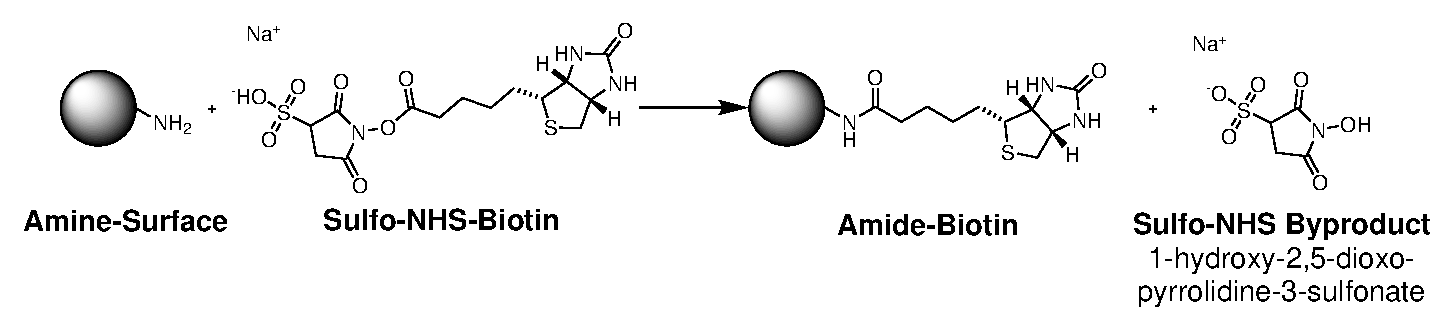
\includegraphics[width=\linewidth]{./Ressources/Chemistry/Sulfo-NHS.eps}
	\capption{Amine Bead Modification with Sulfo-NHS-Biotin}{An amine terminated bead is incubated with sulfo-NHS-Biotin to cover its surface by amide-Biotin. As byproduct the sulfo-NHS-ester 1-hydroxy-2,5-dioxopyrrolidine-3-sulfonate splits off. }
	\label{fig:Chem:NH2-NHS}
\end{figure}


\begin{figure}[htb!]
	\centering
	\subfloat{
		\subfigimg[height=90pt]{a}{./Ressources/Biotinyl/mag-nh2}	
	} \hfill
	\subfloat{
		\subfigimg[height=90pt]{b}{./Ressources/Biotinyl/cooh}	
	}\hfill
	\subfloat{
		\subfigimg[height=90pt]{c}{./Ressources/Biotinyl/IgG-cooh}	
	} \\
\vspace{\baselineskip}
	\subfloat{
	\subfigimg[height=150pt]{c}{./Ressources/Biotinyl/stability}	
	}

	\capption{Titration of Biofunctional Molecules on \SI{8}{\micro\meter} Particles}{ (\textbf{a}) NHS-Biotin, MFI, CV, reduced chi square = 275.19597, Hill Fit $y=Vmax*x^n/(k^n+x^n)$, Vmax = 173.077, k = 0.0572831, n = 1.63554 (\textbf{b}) Amin-PEG$_2$-Biotin MFI, CV, outlier neglected Gleichung: $y=Vmax*x^n/(k^n+x^n)$ Vmax	171,02602, k   	0,04201, n   	0,91338,Chi-Quadr Reduziert	4,07387	(\textbf{c}) MFI, CV, reduced chi square = 0.91011, Hill Fit $y=Vmax*x^n/(k^n+x^n)$, Vmax = 713.83643, k = 182.83011	, n = 0.72458  (\textbf{d}) MFI, SEM, $\tau_{decay}$ = \num{1.42557 +- 0.16188}	Equation	$y = A \exp^\frac{-x}{\tau_{decay}} + y_0$	y0	0.12369 ± 0.01576	A1	0.91263 ± 0.06964	t1	1.42557 ± 0.16188	Reduced Chi-Sqr	0.00542 }
	\label{fig:biotinyl:titration}
\end{figure}



%\begin{figure}[htb!]
%	\centering
%	\includegraphics[width=.7\linewidth]{./Ressources/Biotinyl/IgG-cooh}
%	\capption{Titration of Anti-IgG1 on \SI{8}{\micro\meter} Particles}{MFI, CV, reduced chi square = 
%		0.91011, Hill Fit $y=Vmax*x^n/(k^n+x^n)$, Vmax = 713.83643, k = 182.83011	, n = 0.72458 }
%	\label{fig:biotinyl:IgG-cooh}
%\end{figure}

%\begin{figure}[htb!]
%	\centering
%	\includegraphics[width=\.7\linewidth]{./Ressources/Biotinyl/stability}
%	\capption{Titration of Anti-IgG1 on \SI{8}{\micro\meter} Particles}{MFI, SEM, reduced chi square = 
%		0.00542, Hill Fit $y=Vmax*x^n/(k^n+x^n)$, Vmax = 713.83643, k = 182.83011	, n = 0.72458 }
%	\label{fig:biotinyl:stability}
%\end{figure}


\section{Concentration Measurements in MRCyte}
Explain v-c
\begin{figure}[htb!]
	\centering
	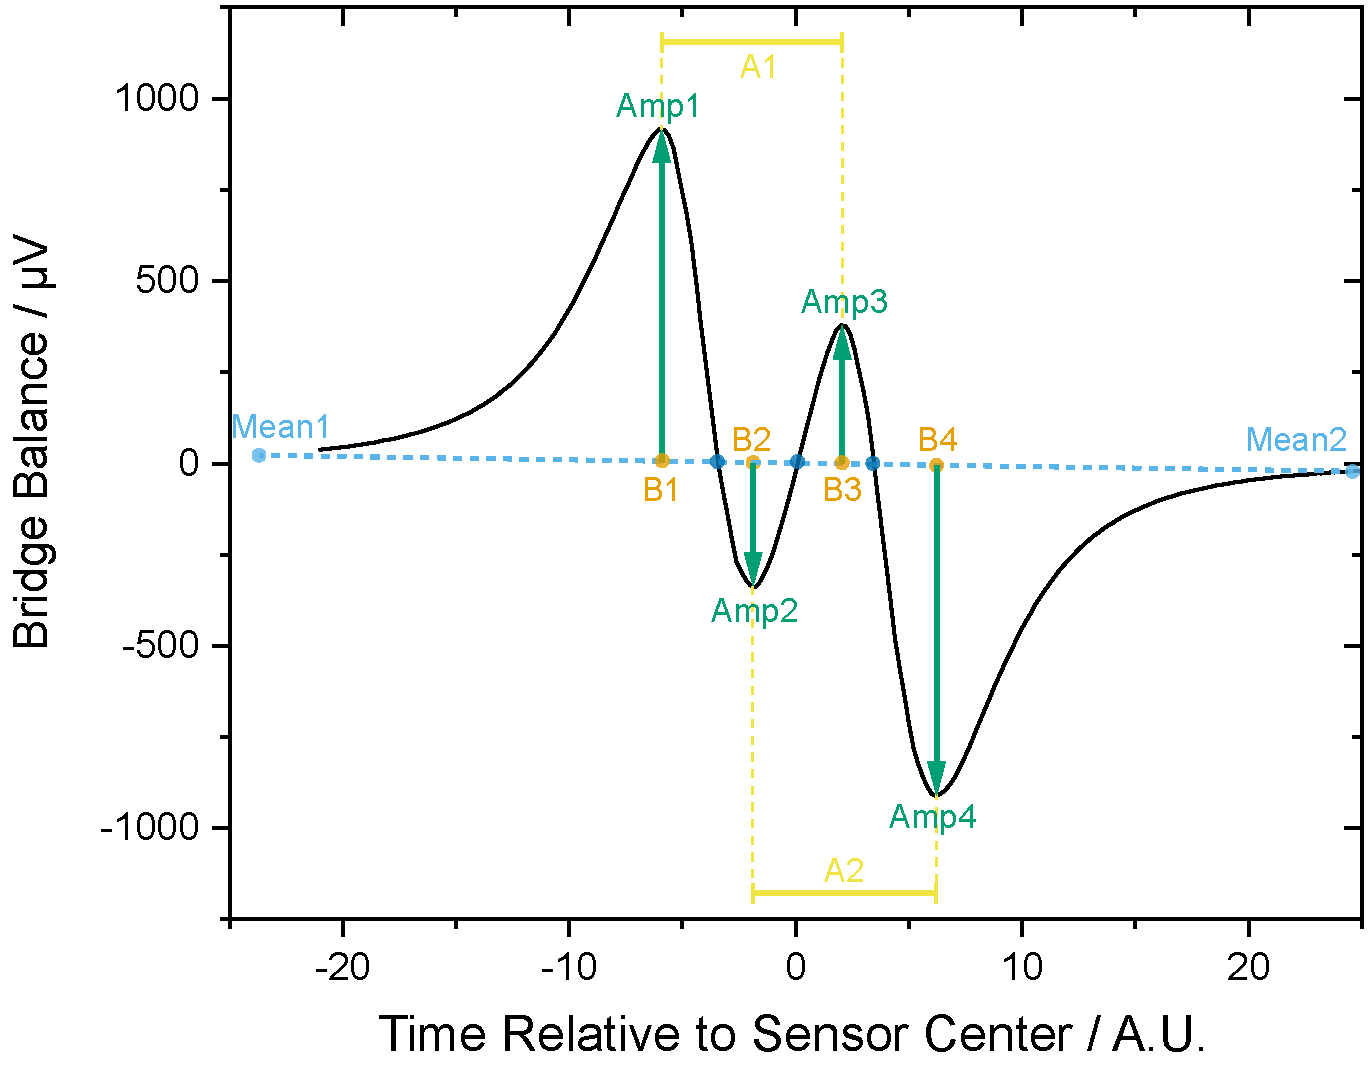
\includegraphics[width=.7\linewidth]{Ressources/Simulation/ExampleSignal}
	\capption{Example Signal of Magnetic Measurement}{explain all}
	\label{fig:conc:example}
\end{figure}

\begin{figure}[htb!]
	\centering
	\includegraphics[width=.7\linewidth]{Ressources/Concentration/Losses-Syringe-Tubing}
	\capption{Bead Loss Evaluation in Connectors}{Losses in different buffers and bead surfaces.}
	\label{fig:conc:losses_syringe}
\end{figure}



\subsection{Calibration of Flow Field}
\begin{figure}
	\centering
	\subfloat{
		\subfigimg[height=150pt]{a}{Ressources/Concentration/ConcentrationError}	
	} \hfill
	\subfloat{
		\subfigimg[height=150pt]{b}{Ressources/Concentration/ConcentrationVelocity}	
	}
	\capption{Absolute Concentration Measurements}{Mean from 3 independent measurements(\textbf{a}) mean, sd (\textbf{b}) mean, SEM, Reference Count based error: Liner fit steepness \num{0,34622 +- 0,00968} --> Correction Factor (inverse) \num{2,88833 +- 0,08075}, Velocity Based Correction: $Q/A$ Dims: \SI{700}{\micro\meter}x\SI{50}{\micro\meter} Q = \SI{30}{\micro\liter\per\minute} --> \num{2,26109}}
	\label{fig:conc:AbsConcError}
\end{figure}

\begin{figure}
	\centering
	\subfloat{
		\subfigimg[height=150pt]{a}{Ressources/Concentration/BiotinylWrongCorrection}	
	} \hfill
	\subfloat{
		\subfigimg[height=150pt]{b}{Ressources/Concentration/BiotinylTime}	
	}
	\capption{Error Sources in Concentration Measurements}{(\textbf{a}) mean, SEM Fit factor comparison with protein coated surfaces (\textbf{b}) mean, SEM}
	\label{fig:conc:BiotnylWrongCorr}
\end{figure}

\subsection{Count Stability}
Measurement over 1h

\begin{figure}[!h]
	\centering
	\subfloat{
		\subfigimg[height=150pt]{a}{Ressources/Concentration/BiotinylCountAll}	
	} \hfill
	\subfloat{
		\subfigimg[height=150pt]{b}{Ressources/Concentration/BiotinylTimeAll}	
	}
	\capption{Reproducibility of Concentration Measurements with Saturated Neutravidin Surface}{(\textbf{a}) \SI{80}{\micro\liter\per\minute} mean, SEM (\textbf{b}) All,mean, SEM,}
	\label{fig:conc:All}
\end{figure}



\begin{figure}[htb!]
	\centering
	\includegraphics[width=.7\linewidth]{Ressources/Concentration/CaptureVelocity}
	\capption{Measured Bead Velocity}{ p < 0.01}
	\label{fig:conc:vel}
\end{figure}




\subsubsection{Concentration Measurement in Diluted Whole Blood}


\begin{figure}[htb!]
	\centering
	\includegraphics[width=.7\linewidth]{Ressources/Concentration/CorrectionBlood}
	\capption{Absolute Concentration Measurement in Blood Samples Under Varying Channel Height}{Velocity Correction does not work for high concentrations in \SI{50}{\micro\meter}}
	\label{fig:conc:blood}
\end{figure}




\subsection{Differential Counting Setup}

\subsubsection{Sensitivity Calibration}

\begin{figure}[!h]
	\centering
	\subfloat{
		\subfigimg[height=150pt]{a}{Ressources/Differential/Optupper}	
	} \hfill
	\subfloat{
		\subfigimg[height=150pt]{b}{Ressources/Differential/Optlower}	
	}
	\capption{Hysteresis Calibration for Stacked \Gls{pcb} }{(\textbf{a}) Optimized for top sensor (\textbf{b}) Optimized for bottom sensor}
	\label{fig:diff:sensitivity}
\end{figure}

\subsubsection{Concentration Measurement in Buffer Solution}



\begin{figure}[!h]
	\centering
	\subfloat{
		\subfigimg[height=150pt]{a}{Ressources/Differential/Bottom}	
	} \hfill
	\subfloat{
		\subfigimg[height=150pt]{b}{Ressources/Differential/Top}	
	}
	\capption{Flow Rate Dependency of Counting Setup}{(\textbf{a}) Optimized for top sensor (\textbf{b}) Optimized for bottom sensor}
	\label{fig:diff:flowRate}
\end{figure}

\begin{figure}[htb!]
	\centering
	\includegraphics[width=.7\linewidth]{Ressources/Differential/Differential}
	\capption{Optimal Differential Counting Flow Rate}{Losses in different buffers and bead surfaces.}
	\label{fig:conc:optimum}
\end{figure}




\subsection{Surface Magnetization of Biofunctionalized Beads}

Somehow BNF-Dextran showed unspeficity initally, but not anymore later on

\begin{figure}[!h]
	\centering
	\subfloat{
		\subfigimg[height=150pt]{a}{Ressources/Concentration/BNFC1}	
	} \hfill
	\subfloat{
		\subfigimg[height=150pt]{b}{Ressources/Concentration/BNFVc}	
	}
	\capption{Bead Coverage Assay with BNF-Dextran-redF-\SI{100}{\nano\meter}}{(\textbf{a}) 1. \SI{80}{\micro\liter\per\minute} 2. \SI{40}{\micro\liter\per\minute} 3. \SI{20}{\micro\liter\per\minute} 4. \SI{10}{\micro\liter\per\minute} (\textbf{b}) d = \SI{8}{\micro\meter}}
	\label{fig:conc:BNF}
\end{figure}



\begin{figure}[!h]
\centering
\subfloat{
	\subfigimg[height=150pt]{a}{Ressources/Concentration/OceanC1}	
} \hfill
\subfloat{
	\subfigimg[height=150pt]{b}{Ressources/Concentration/OceanVc}	
}
\capption{Bead Coverage Assay with OceanNanotec \SI{50}{\nano\meter}}{Mean from 3 different particle distributions at maximum coverage, SEM(\textbf{a}) d = \SI{4}{\micro\meter} (\textbf{b}) d = \SI{8}{\micro\meter}}
\label{fig:conc:Ocean}
\end{figure}


\section{Surface Modification and Biofunctionalization of the Sensor Chip Substrate}

\subsection{Physisorption}
Quantification in Plate Reader
Trial with Neutravidin + Sensor (Esthis Versuch)
\clearpage

\begin{figure}
	\centering
	\includegraphics[height=150pt]{Ressources/ResultPlots/SurfaceFuncSiNAlOx}
	\capption{Surface Adsorption Stability of Neutravidin on \Gls{sin} and \Gls{alox}}{Blank with PBS and Blank substrate, corrected, then normalized, absolute protein per \textasciitilde \SI{25}{\milli\meter\square}}
	\label{fig:unsp:wash}
\end{figure}


\subsection{Covalent Attachment}
%\clearpage


\begin{figure}[htb!]
	\centering
	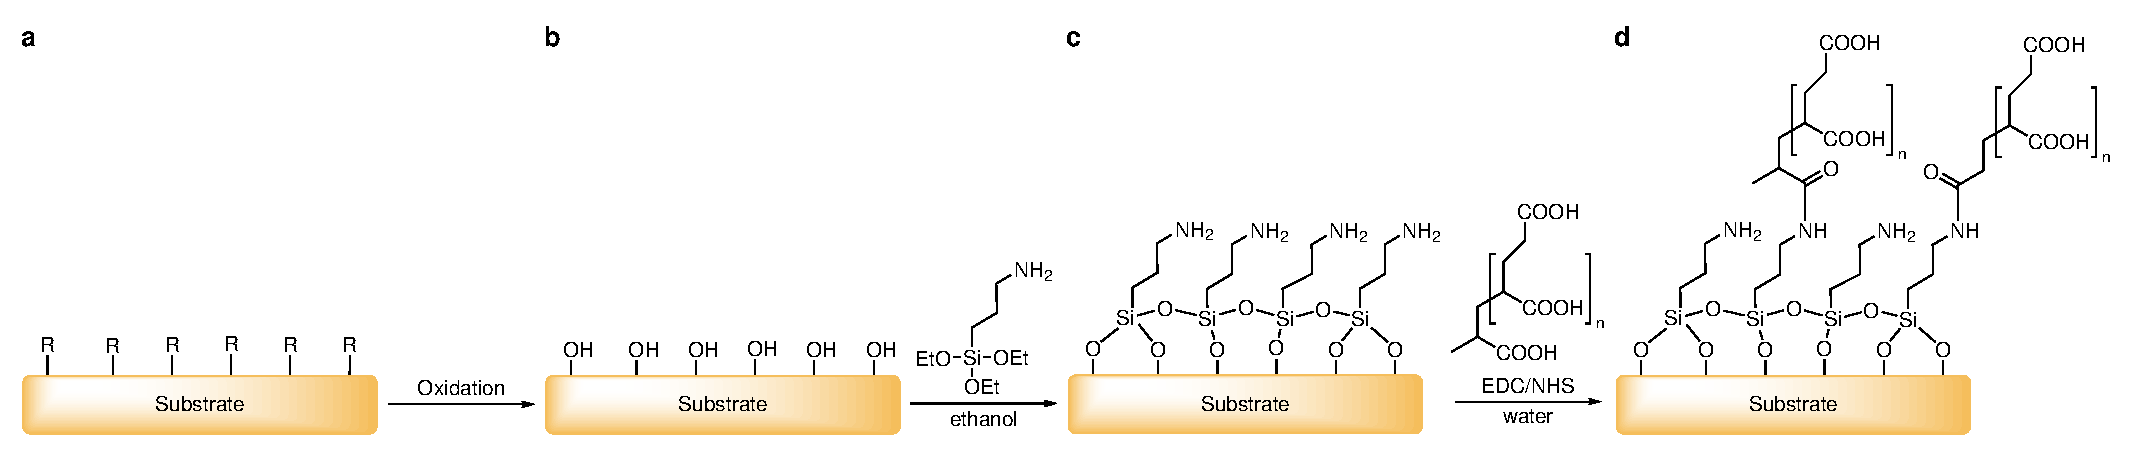
\includegraphics[width=1\linewidth]{Ressources/Chemistry/Substrate}
	\capption{General process chain of chemical surface modification}{Any substrate with various surface groups R (\textbf{a}) is oxidized to exhibit \gls{hydroxyl} groups.(\textbf{b}). Then a silane \gls{sam} is attached (\textbf{c}) and subsequently modified by carbodiimide chemistry with \gls{paa}. (\textbf{d})}
	\label{fig:chem:func:withPAA}
\end{figure}


\begin{figure}[!h]
	\centering
	\subfloat{
		\subfigimg[height=150pt]{a}{Ressources/Covalent/SerpentinesDensityCount}	
	} \hfill
	\subfloat{
		\subfigimg[height=150pt]{b}{Ressources/Covalent/NeutravidinTitration}	
	}
	\capption{Neutravidin Titration Fluorescence and Bead Capture Assay}{Relate count to area, then change MFI to counts \si{\per\micro\liter\per\milli\meter\squared}(\textbf{a}) Serpentine (\textbf{b}) Glass}
	\label{fig:coval:fluo}
\end{figure}

\subsubsection{Plasma-Based Approach}
\begin{figure}
	\centering
	\includegraphics[height=150pt]{Ressources/ResultPlots/PDMS-sessileDrop}
	\capption{Hydrophbicity Analysis of \gls{pdms} under Plasma Exposure}{test123}
	\label{fig:coval:plasma}
\end{figure}


\subsubsection{Water-Based Approach}
Sonicate in Acetone and Water 5'
1:1 \gls{hcl}:Methanol
\gls{h2so4}
Treat for 30 min in light boiling water
\chapter{Discussion}
Start by briefly summarizing your major findings, but without repeating exact data from the Results. This makes your novel information clear to peer reviewers and, later on, readers. It also forces you to decide which findings you should focus on in the Discussion.
Thereafter, discuss possible underlying mechanisms. Why did you get these results, what is happening? Mechanisms, particularly molecular mechanisms, have very high “impact” in the natural sciences.

Next, compare your findings to those of other relevant publications and attempt to explain any discrepancies. If your findings disagree with those of others in the area, compare their publication to your own manuscript in minute detail, looking for any differences (especially in methodology) that might explain the discrepancy.

Consider the possible limitations of your own study—paradoxically, most reviewers consider an awareness and openness about potential weaknesses as a strength. However, do not forget to emphasize strengths as well.

Discuss the possible consequences of your observations and/or future investigations required or motivated. Be as concrete as possible about future perspectives. As in the abstract, writing the equivalent of “more research is needed” is meaningless—more research is always needed. Describe the hypotheses, questions or mechanisms that need to be investigated and/or methods that should be applied, concretely and concisely. And, of course, if your research findings have potential practical implications, discuss these in some detail as well.

Finally, state your conclusions—have you supported or rejected the hypothesis you posed, or obtained an answer to your research question?





eriving Navier-Stokes equation by the Cauchy momentum equation is complex and harbors several sources of error. First, an incompressible Newtonian fluid as well as channel boundary is assumed. The used water suspensions are approximated with negligible compressibility, which is not true for the real case. Also, for blood or other shear-thinning fluids these deviations are prone for high errors.  

Then, the divergence relation of the respective viscous stress (eq. \ref{eq:divergence_Stresstensor}) does not hold for non-uniform viscosity $\eta$.

For later studies in a matlab model, the flow velocity and shear stress computations were carried out with the error sources considered. 


--> signal analysis with wavelet analysis

Third, the transient term (eq. \ref{eq:navierstokes}) was neglected in all simulations, but a connected syringe pump possesses a slow rise time (Fig. \ref{fig:fluidic:pumpStability:transient}) and a remaining ``pulsation error'' in steady state (Fig. \ref{fig:fluidic:pumpStability:steadystate}). In effect, another error adds to the simulation, which is only valid after several ten seconds of the last flow rate change.
\begin{figure}
	\begin{subfigure}[b]{0.5\textwidth}
		\centering
		\addtocounter{subfigure}{1}  
		\subfigimg[clip,trim=115 100 80 60, height=100pt]{a} {./Ressources/Fluidic/Transient_SyringePump.jpg}		
		\addtocounter{subfigure}{-1}  
		\phantomsubcaption
		\label{fig:fluidic:pumpStability:transient}
	\end{subfigure}%
	\begin{subfigure}[b]{0.5\textwidth}
		\centering
		\addtocounter{subfigure}{1}  
		\subfigimg[height=100pt]{\textbf{b}}{./Ressources/Fluidic/SyringeSteadyState.eps}
		\addtocounter{subfigure}{-1}  
		\phantomsubcaption
		\label{fig:fluidic:pumpStability:steadystate}
	\end{subfigure}
	\capption{Syringe Pump error sources}{Set flow rate: \orangeline, Real Flow Rate: \blueline \subref{fig:fluidic:pumpStability:transient} Transient step answer of a syringe pump through a microtube with \SI{254}{\micro\meter} inner diameter. \subref{fig:fluidic:pumpStability:steadystate} Steady state flow rate error around the desired \SI{5}{\micro\liter\per\minute} dispensing rate. A sinusoidal behaviour caused by the microstepping can be observed. \cite{lit:fluidic:fluigentPumpStability}}
	\label{fig:fluidic:pumpStability}
\end{figure}


Second, the channel height varies in reality as a result of fabrication inaccuracies. 

modification of nh2 with paa and protein like cooh

Contact angle for silanization of surface methods more useful --> should be 1st approach for characterization

Anti-Biotin-PE working?
BNF-Dextran-Streptavidin unspecific binding?
electrostatic surface interaction
evidence covalent binding?

gas bubbles, adsprotion decrease, tubing exchange
activity of protein

bead rolling with biotin-cooh, biotin-nh2, plain-cooh, plain-nh2 --> velocity correction factor

concentration of beads in differential setup too high, maybe better results with lower.
\chapter{Outlook}
The validated protocols in this thesis for bead and surface bio-functionalization present a comprehensive groundwork for further experiments regarding affinity measurements, magnetic bead or cell trapping, and exosome assays. Also, a computational and practical model for the cell receptor density has been characterized extensively and could be used for a further study of the magnetic flow cytometer or even as internal standard in assay development. 

The whole magnetic flow cytometer, nevertheless, offers some elements for potential improvements: \\
First, the chip design could be tailored more to the respective sensor application in order to achieve beneficial flow patterns, less bead losses, or the filtering of bubbles.\\
Second, the photo-lithographic sensor design could be improved by its sensitivity for each beads and cells. The distance between \gls{gmr}-bridges could be increased for an enhanced resolution of time-of-flight and peak overlap with the compromise of a further limited, measurable concentration. Also, whereas cells require high sensitivity and low noise along with magnetic focusing, magnetic beads could be measured with a channel spanning \gls{gmr}-setup to avoid the additional complexity of the magnetophoretic nickel-iron structures. Especially in the light of highly sensitive single-molecule or affinity measurements, the \acrlong{mr} could be leveraged by exploiting the tunnel-magneto-resistance instead of the giant-magneto-resistance in a new sensor layout.\cite{lit:GMRTMR}\\
Third, from a time- and work-efficiency perspective, it could be profitable to develop a (real-time, automatized) data analysis software by a model-based wavelet correlation or compressive sensing. Several algorithms have already been developed \cite{lit:thes:michaelBauer}, however, experimental verification and overall back-end integration is required.\\
Lastly, the bio-functionalization could be benchmarked for its attachment mechanism from a chemistry and physical standpoint by field-typical methods such as dynamic-light scattering, activity assays, electron/atomic-force microscopy, or spectroscopy. This would provide deeper insights into surface composition and hence the covalent to physisorption efficiency or model parameters for the bead rolling.\\
Experimentally, several pathways can now be explored. The bead rolling and its subsequent motion inside a plain channel could be related its electrostatic surface interaction by testing for example \gls{carboxyl}, \gls{amine}, and biotinylated particles as well as their intermediates. Also a more precise velocity correction factor could be formulated.\\

Also, the differential counting setup should not be omitted prematurely. By removing the tubing interconnection, for instance by a through silicon via combined with a micrometer thin \gls{pdms} sheet, many losses could be lowered. Further sequential interrogation of affinity measurements can be explored over a single permanent magnet as excitation field. Moreover, the utilized high bead concentrations did probably not reflect the ultimate capabilities during a time-of-flight measurement. However, the current cost-benefit ratio for the complex technological and time-related efforts needed to create this setup constitutes to a strong opposition to further development. An in-plane integration of the workflow seems to be more reasonable.

Despite the elaborated improvement options, the magnetic flow cytometry system starts to open a new field in clinical diagnostics and point-of-care testing, where a measurement is completely independent from the optical background of blood samples. With the proper integration level, tests for immune cell counts or inflammation intensities\footnote{measured by the cell marker density and the subsequent adhesiveness to an antibody-functionalized surface} could be performed bedside in minutes and effectively start saving lives in the near future. 





 % Abkürzungsverzeichnis
\glsaddall
\printacronyms[title={List of Abbreviations}]
%\printglossaries
\addxcontentsline{toc}{chapter}{List of Abbreviations}
\clearpage
\newpage\null\thispagestyle{empty}\newpage
\listoffigures % Abbildungsverzeichnis
\addxcontentsline{toc}{chapter}{List of Figures}


\listoftables % Tabellenverzeichnis
\addxcontentsline{toc}{chapter}{List of Tables}
\clearpage
\newpage\null\thispagestyle{empty}\newpage
\nocite{*}	% stellt alle Quellen dar, auch die, die nicht zitiert wurden
%\bibliographystyle{plain}

\addxcontentsline{toc}{chapter}{Bibliography}
\printbibliography
\clearpage
%\newpage\null\thispagestyle{empty}\newpage
\addxcontentsline{toc}{chapter}{Statement}
\thispagestyle{empty}
\chapter*{Statement}
I declare that I have authored this thesis independently, that I have not used other than the declared
sources / resources, and that I have explicitly marked all material which has been quoted either
literally or by content from the used sources. 

\vspace{18.1mm}
\rule[-3.7mm]{\linewidth}{0.5pt}
\Ort{}, \Datum{}, Johann Alexander Brenner

\end{document}
